\chapter{System Detail}
\label{sec:chapter4}
In this chapter, we define in detail the system we develop to solve to implement the method described Sec. \ref{sec:solution}. The system is composed of five main modules and each of them addresses a specific requirement imposed by our solution. We report the functionalities of each module, describing also the algorithms we implement and the technologies used for their construction. These modules are the following:

\begin{enumerate}
	\item \textbf{Doors Detector:} this module implements the main requirement of this thesis: the development of a doors detector for indoor autonomous robots. We approach the problem of finding doors as an object detection task, that we address using a deep learning technique. Doors detector is implemented through DETR \cite{detr}, a deep end-to-end architecture to perform object detection. To better understand how DETR works, we provide an overview of the principal machine learning and deep learning principles. Finally, we described in detail the DETR's architecture. 
	\item \textbf{Simulation Environment:} the second part of our system is the simulation environment used to collect the dataset. As described in Sec. \ref{sec:importanceofsimulation}, simulation is widely used in robotic applications, so we employ this technique to collect the dataset for training the doors detector. The acquisition of the doors dataset solves the lack of suitable datasets for robotic applications, as explained in Sec. \ref{sec:goals}. We choose Gibson \cite{gibson} as the virtualization framework and Matterport3D \cite{matterport} as the worlds' dataset. In the dedicated section, we describe the main functionalities of Gibson and Matterport3D. Then, we report the issues of these technologies that prevent correct and fast data collection. We finally explain the adopted solution to overcome these limitations: we developed a modified version of Gibson that implements a new simulation stage in which the robot can be placed freely in any location.
	\item \textbf{Pose Estimator:} this module emulates a possible navigation strategy used by a real autonomous agent and extracts  the locations from which the data points are collected. Thanks to this module unified with the new version of Gibson, we offer a method to easily acquire a visual dataset which models the \textit{open-set} conditions in which an autonomous agent operates. In this section, we report the underlying algorithms implemented in this component.
	\item \textbf{Dataset Manager:} another important aspect of the system provided by this thesis is the dataset. We report in detail by which data it is composed, describing also the labeling procedure. In addition, we mention the framework we developed for managing the dataset.
	\item  \textbf{Model Evaluator:} the last component of our system aims to evaluate the model's performance. As reported in Sec. \ref{sec:solution}, we propose a new metric that considers also the negative images (examples with no objects of interest). For this module, we describe the metric we propose and the procedure to obtain its results.
\end{enumerate}


\section{Doors Detector}
\label{sec:doors_detector}

The doors detector we propose is built with DETR \cite{detr}. The module we develop is public available on Github, in the main repository\footnote{The main thesis's repository: \url{https://github.com/micheleantonazzi/master-thesis-robust-door-detector}.} of this thesis inside the \textsf{doors-detector} package. In this section, we describe in detail the architecture and the loss functions of DETR.

\subsection{DETR}
\label{sec:detr}
The doors detector proposed by this thesis is based on DETR \cite{detr} (DEtection TRansformer), a novel deep approach to perform object detection.  In DETR, the object detection problem is modeled as a direct \textit{set prediction}, making the detection pipeline a simple end-to-end unified architecture. Modern detectors address this set prediction in an indirect way using hand-crafted algorithms based on a large set of proposals \cite{yolo} or anchors \cite{focalloss}. Their performances are significantly influenced by these post-processing steps to collapse near-duplicate predictions, like non-maximum suppression or anchor generation. The first important aspect of DETR  is its architecture (explained in Sec. \ref{sec:detrarchitecture}). DETR uses a Transformer to find complex relationships between features extracted in the same image. In this way, the model reasons about the whole image context without considering any form of prior knowledge about the task. The second important aspect to address the set prediction problem is the loss functions (described in \ref{sec:detrlosses}). DETR uses a set loss function that performs bipartite matching between predicted and ground-truth objects.

\subsubsection{DETR Architecture}
\label{sec:detrarchitecture}
The architecture of DETR (reported in Fig. \ref{fig:detrarchiecture}) consists of three main components: a backbone convolutional neural network (CNN) for features extraction, an encoder-decoder transformer to capture the relationships between the extracted features, and a simple feed-forward network (FFN) that makes the final detection: the coordinates of the bounding boxes and their relative labels.

\begin{figure}[h!]
	\centering
	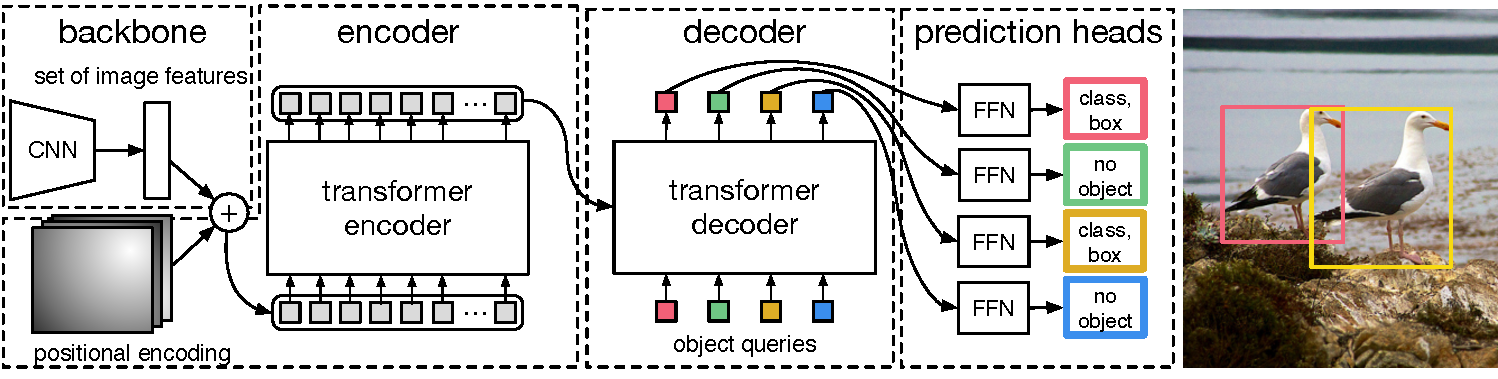
\includegraphics[width=\linewidth]{images/detrarchitecture.pdf}
	\caption{The architecture of DETR. It uses a conventional CNN backbone to learn a 2D representation of an input image. Then, this representation is flattened and encoded before being passed into the transformer encoder. The transformer decoder then takes as input a small fixed number of learned positional embeddings, called \textit{object queries}, and additionally attends to the encoder output. Finally, each output embedding of the decoder is processed by a  simple feed-forward network (FFN) that predicts either a detection (class and bounding box) or a ``no object'' class. Image from \cite{detr}.}
	\label{fig:detrarchiecture}
\end{figure}
\newpage
\paragraph{CNN Backbone} The first element in DETR's architecture is a CNN backbone.  Ideally, any backbone can be used depending upon the complexity of the task to provide a low dimensional representation of the image extracting features from it. Starting from the initial image $x_{img} = \R^{3\times H_0\times W_0}$ (with 3 color channels and dimensions $H_0$, $W_0$), a conventional CNN backbone generates a lower-resolution activation map $f \in \R^{C \times H \times W}$. Typical values used in this paper are $C = 2048$ and $H, W = \frac{H_0}{32}, \frac{W_0}{32}$. 

A ResNet (residual network) \cite{resnet} is used as CNN backbone to deal with the issues introduced by the vanishing gradient problem. It makes deep neural networks difficult to train and optimize: when a network's depth increases, accuracy gets saturated and then degrades rapidly. This unwanted situation is called \textit{degradation} of training accuracy. Unexpectedly, such degradation is not caused by overfitting, and adding
more layers to a deep model leads to higher training error. The authors address the degradation problem by introducing a \textit{deep residual learning} framework, commonly called ResNet. The proposed method is based on the insight that a few overlapping layers can fit a residual mapping instead of directly fitting a desired underlying mapping. This principle is formalized as follows. Let $\mathcal{H}(x)$ be the desired underlying mapping fit by a few stacked layers (not necessarily the entire net), where $x$ denotes the inputs of the first layer. Since multiple non-linear layers can approximate non-linear functions, then  the same layers can approximate the residual functions $\mathcal{H}(x) - x$. The authors of ResNet \cite{resnet} let these layers approximate a residual function
$\mathcal{F}(x) := \mathcal{H}(x) - x$, so that the original function becomes
$\mathcal{F}(x)+x$. The authors hypothesize that it is easier to optimize the residual mapping than to optimize the original unreferenced mapping.  If the optimal function is closer to an identity
mapping than to a zero mapping, it should be easier for the
solver to find the perturbations with reference to an identity
mapping, than to learn the function as a new one. This means that subsequent blocks in our network are thus responsible for fine-tuning the output of a previous block, instead of having to generate the desired output from scratch.

\begin{figure}[h!]
	\centering
	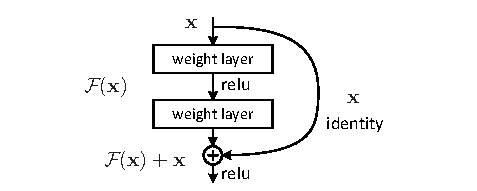
\includegraphics[width=\linewidth]{images/residualblock.pdf}
	\caption{Residual learning: a building block. The formulation of $\mathcal{F}(x)+x$ can be realized with a ``shortcut connection'', that skips one or more layers. Image from \cite{resnet}.}
	\label{fig:resblock}
\end{figure}

\paragraph{Transformer Encoder-Decoder} The second part of DETR is a Transformer \cite{transformer}, a sequence-to-sequence (Seq2Seq) architecture that transforms a given sequence of elements, such as the sequence of words in a sentence, into another sequence. Recent studies \cite{surveytransformer} demonstrate the effective application of Transformer in Computer Vision. By using a Transformer model, DETR globally reasons about all objects together using pair-wise relations between them, thus being able to use the whole image as context. In this way, DETR predicts (in a single pass) a set of objects and
models their relations. Since DETR performs object detection, the Transformer's input is a sequence of features extracted from an image.

The Transformer model, proposed by \citeauthor{transformer} \cite{transformer}, is the first transduction model relying entirely on self-attention mechanism to compute representations of its input and output without using RNNs or convolutions. Self-attention is an attention mechanism that relates every single element in a sequence with the other elements and finally computes a representation of the entire sequence. In other words, the attention mechanism decides at each step which parts of the sequence are important by assigning a weight to each element. The Transformer architecture (Fig. \ref{fig:transformerarc}) is based on an encoder-decoder structure. In a general way, the encoder maps an input sequence of symbol representations $(x_1, ..., x_n)$ into a sequence of continuous representations $z = (z_1, ..., z_n)$. Given $z$, the decoder then generates an output sequence $(y_1, ..., y_m)$ of symbols one element at a time.

More specifically, the Transformer's encoder  is composed of a stack of $N = 6$ identical layers. Each layer has two sub-layers: the first is a multi-head self-attention mechanism and the second is a simple, position-wise fully connected feed-forward network. The authors add a residual connection (like ResNet \cite{resnet}) around each sub-layer, followed by layer normalization. The output of each sub-layer is $LayerNorm\big(x + Sublayer(x)\big)$. The decoder is also composed of a stack of $N = 6$ identical layers. Each of them has the same sub-layers of the encoder with a third one that performs multi-head attention over the output of the encoder stack. The authors modify the self-attention
sub-layer in the decoder to prevent positions from attending to subsequent positions. This masking, combined with fact that the output embeddings are offset by one position, ensures that the predictions for the position $i$ can depend only on the known outputs at positions less than $i$.

\begin{figure}[h!]
	\centering
	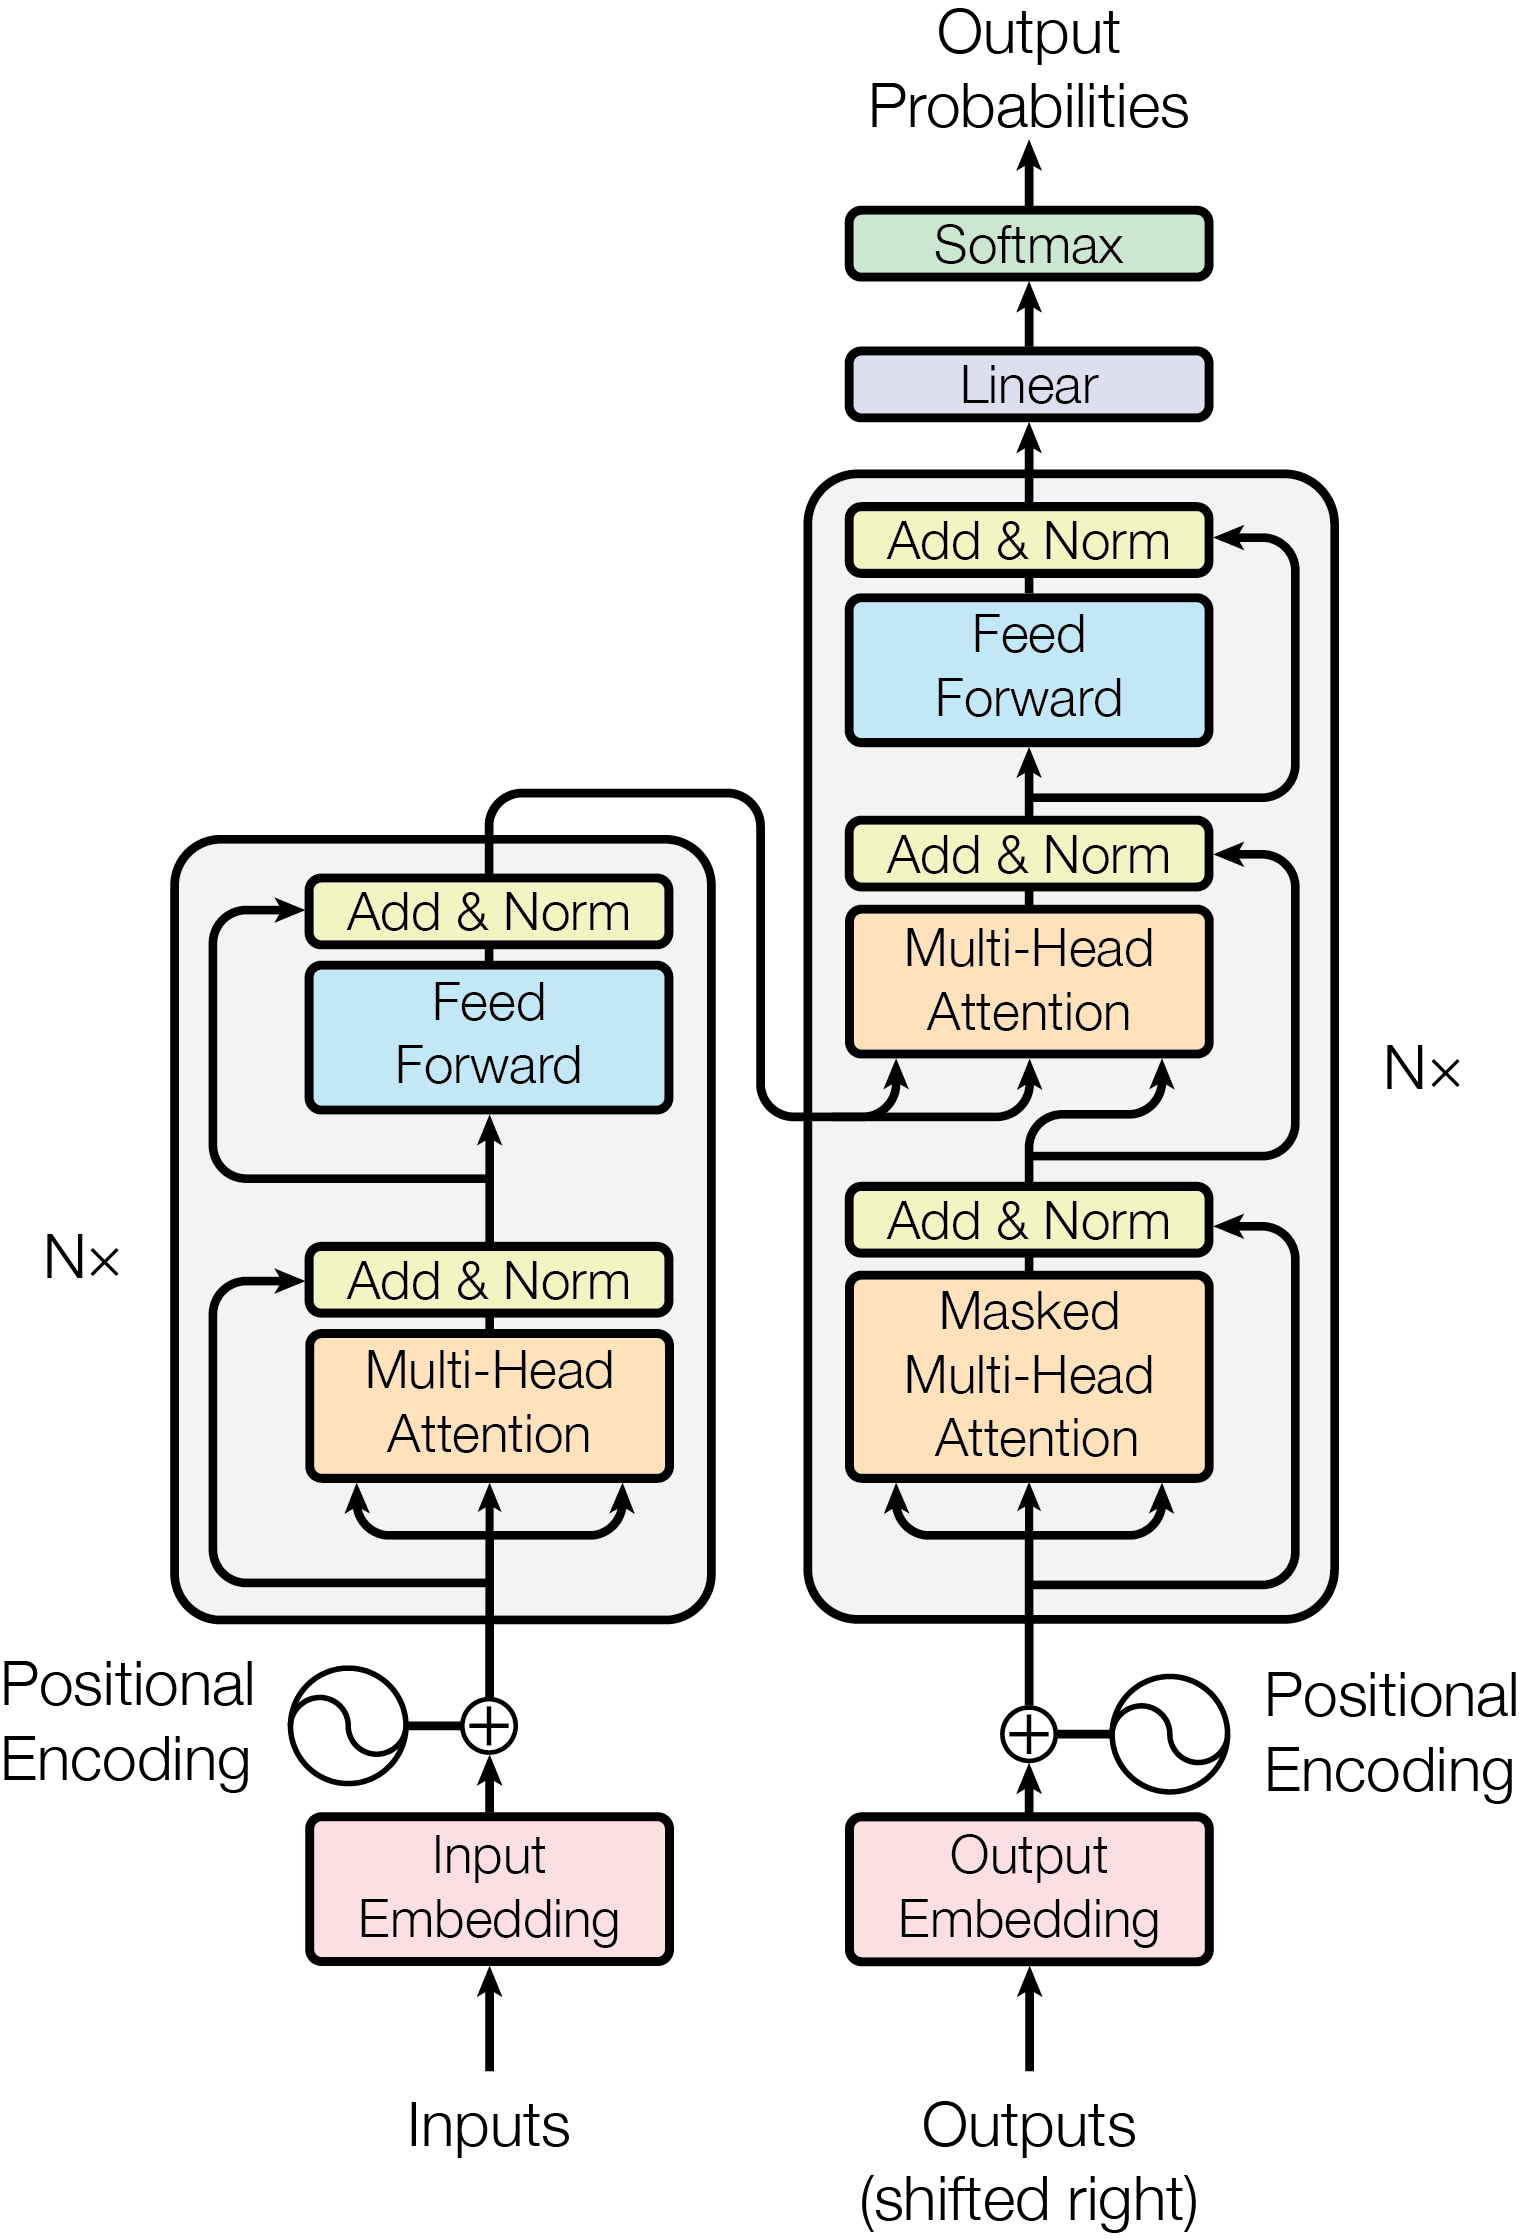
\includegraphics[width=0.8\linewidth]{images/transformerarchitecture.png}
	\caption{The Transformer model architecture. Image from \cite{transformer}.}
	\label{fig:transformerarc}
\end{figure}

DETR \cite{detr} uses a standard Transformer developed for natural language process as proposed in \cite{transformer}. The high-level activation map $f$ extracted from the CNN backbone is rescaled from $C$ to a smaller dimension $d$ by a $1\times1$ convolution. The new feature map fed into the Transformer's encoder is $z_0 \in \R^{d, H, W}$. Since the encoder requires a sequence as input, the feature map $z_0$ is collapsed the spatial into one dimension, resulting in a $d\times HW$ feature map. The decoder transforms $N$ embeddings of size $d$.  The difference with the original Transformer \cite{transformer} is that DETR decodes the $N$ objects in parallel at each decoder layer. These input embeddings (called \textit{object queries}) are positional encoding vectors learned by the model during the training phase. They are passed to the input of each attention layer. Since the decoder is permutation-invariant, the $N$ input embeddings must be different to produce different results. Each object query is transformed into an output embedding by the decoder. The number of object queries is a hyper-parameter and it must be greater than the quantity of different objects in an image.

\paragraph{Feed-Forward Networks} The $N$ object queries produced by the decoder are  independently classified into box coordinates and class labels by
a feed-forward network, resulting in $N$ final object predictions. The final predictor is composed of a 3-layer perceptron and a linear projection layer. The perceptron predicts the normalized center coordinates, height, and width of the bounding boxes while the linear layer predicts the class labels. Since DETR predicts a
fixed-size set of $N$ bounding boxes, where $N$ is much larger than the
actual number of objects of interest in an image, an additional special class label $\varnothing$ is used to represent that no object is detected within a slot (it indicates the ``background'' class).

\subsubsection{DETR Loss Functions}
\label{sec:detrlosses}

DETR \cite{detr} simplifies the detection pipeline by dropping multiple hand-designed components that encode prior knowledge, like spatial anchors or non-maximal suppression. To address set prediction in a fully end-to-end way, DETR uses a novel loss function, called \textit{object detection set prediction loss}, that produces
optimal bipartite matching between predicted and ground-truth objects, considering both the class labels and the bounding boxes.

\paragraph{Object Detection Set Prediction Loss} DETR \cite{detr} infers a fixed-size set of $N$ predictions through the $N$ object queries produced by the Transformer's decoder. It is important that $N$ is significantly larger than the maximum number of objects in every image. One of the main difficulties of training is to score predicted objects, by considering the class, position, and size, with respect to the ground-truth. The authors propose a loss function that produces
an optimal bipartite matching between predicted and ground-truth objects considering object-specific (bounding box) losses. 

\begin{figure}[h!]
	\centering
	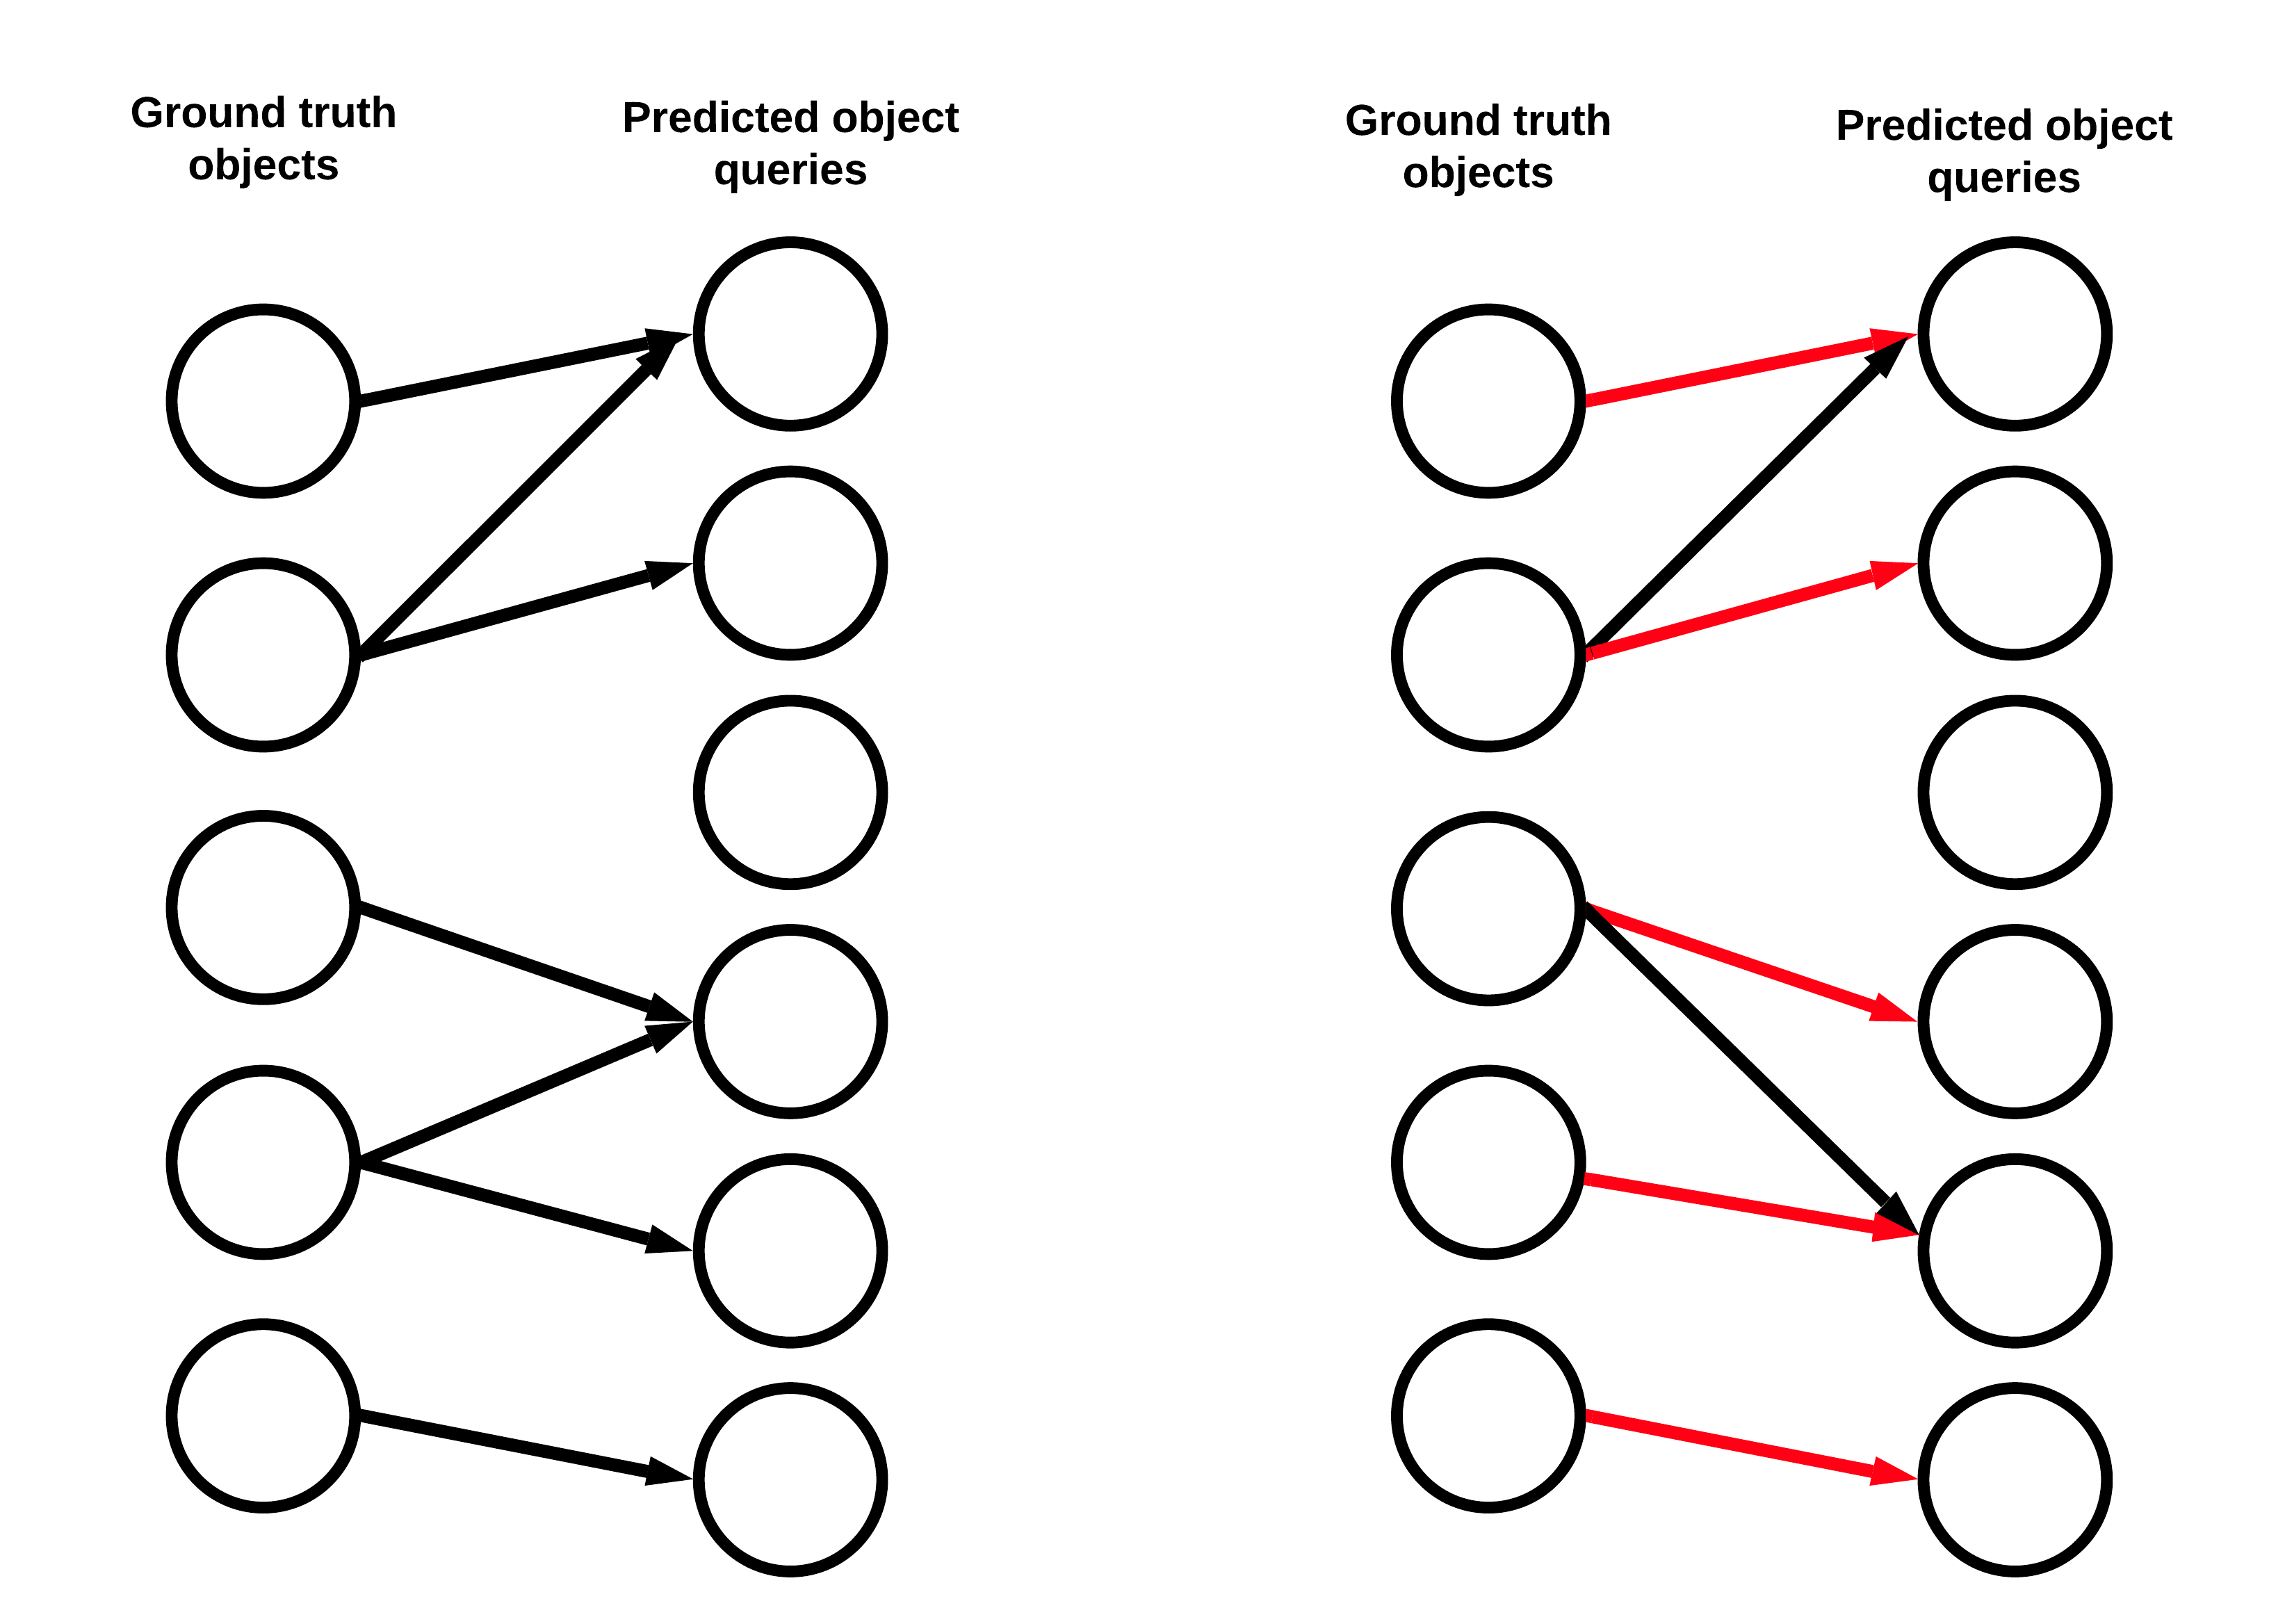
\includegraphics[width=0.9\linewidth]{images/bipartitematching.png}
	\caption{A matching in a bipartite graph. It consists of a set of edges chosen in such a way that no two edges share an endpoint. The loss function $\hat \sigma$ (Eq. \ref{formula:bipartitematching}) finds the best match with the lowest cost between the predicted bounding boxes and the ground-truth objects.}
	\label{}
\end{figure}

Let $y$ be the ground-truth set of objects, and $\hat y = \{\hat y_i\}^{N}_{i = 1}$ the set of $N$ predictions. The bipartite matching between these two sets is the best permutation $\hat \sigma \in \mathcal{G}_N$ of $N$ elements with the lowest cost:

\begin{equation}
\label{formula:bipartitematching}
\hat \sigma = \argmin_{\sigma \in \mathcal{G}_N} \sum_{i}^{N} \mathcal{L}_{match}(y_i, \hat y_{\sigma(i)}),
\end{equation}
where $\mathcal{L}_{match}(y_i, \hat y_{\sigma(i)})$ is a pair-wise \textit{matching cost} between  ground-truth $y_i$ and a prediction with index $\sigma(i)$. This optimal assignment is computed efficiently
with the Hungarian algorithm \cite{hungarian}. The matching cost takes into account both the class prediction and the similarity between predicted and the ground-truth bounding boxes. Each element $i$ can be seen as $y_i = (c_i
, b_i)$, where $c_i$
is the target class label (which may be $\varnothing$) and $b_i \in [0, 1]^{4}$
is a vector that defines ground-truth box coordinates and dimensions. For the
prediction with index $\sigma(i)$, the probability of class $c_i$ is defined as $ \hat p_{\sigma(i)}(c_i)$ and
the predicted box as $\hat b_\sigma(i)$. With this notation, the authors define the matching cost as

\begin{equation}
	\label{eq:detr_hungarian}
	\mathcal{L}_{match}(y_i, \hat y_{\sigma(i)}) = -\mathds{1}_{\{c \neq \varnothing\}}\hat p_{\sigma(i)}(c_i) + \mathds{1}_{\{c \neq \varnothing\}}\mathcal{L}_{box}(b_i, \hat b_{\sigma(i)}),
\end{equation}
which performs one-to-one matching for direct set prediction without duplicates. 

The next step is to compute the loss function, called \textit{Hungarian loss}, for all pairs matched in the previous step. It is a linear combination of a negative log-likelihood for class prediction and a box loss defined later:

\begin{equation}
\label{eq:detr_loss}
\mathcal{L}_{\text{Hungarian}}(y, \hat y) = \sum_{i = 1}^{N} \bigg [-\log \hat p_{\hat\sigma(i)}(c_i) + \mathds{1}_{\{c \neq \varnothing\}}\mathcal{L}_{box}(b_i, \hat b_{\hat\sigma(i)}) \bigg ]
\end{equation}
where $\hat \sigma$ is the optimal assignment computed in Eq. \ref{formula:bipartitematching}. In practice, the authors
down-weight the log-probability term when $c_i = \varnothing$ by a factor 10 to account for class imbalance. 

\paragraph{Bounding Box Loss} The second part of the matching cost in the Hungarian loss is $\mathcal{L}_{box}(\cdot, \cdot)$ that scores the bounding boxes. The authors of DETR \cite{detr} perform box predictions directly without any initial guesses using the $\ell_1$ loss. In our context, this loss measures the distance between the  ground-truth bounding box ($b_i$) and the best predicted box ($\hat b_{\sigma(i)}$) through the L1 norm:

\begin{equation}
\ell_1(b_i - \hat b_{\sigma(i)}) = ||b_i - \hat b_{\sigma(i)}||_1.
\end{equation}

While such an approach simplifies the implementation, the $\ell_1$ loss will have different scales for small and large boxes even if their relative error is similar. To mitigate this issue, the final $\mathcal{L}_{box}(\cdot, \cdot)$ is a linear combination of the $\ell_1$ loss and the generalized IoU loss \cite{generalizediou} $\mathcal{L}_{iou}(\cdot, \cdot)$, that is scale-invariant because it is the ration between the intersection and the union as between a predicted and a ground-truth bounding boxes. The final bounding box loss is:

\begin{equation}
\label{eq:bounding_box_loss}
\mathcal{L}_{box}(b_i, \hat b_{\sigma(i)}) = \lambda_{iou}\mathcal{L}_{iou}(b_i, \hat b_{\sigma(i)}) + \lambda_{L1}||b_i - \hat b_{\sigma(i)}||_1,
\end{equation}
where $\lambda_{iou}$ and $\lambda_{L1}$ are hyper-parameters.

\section{Simulation Environment}

In this section, it is described the method we propose to build the doors dataset. As mentioned in Sec. \ref{sec:importanceofsimulation}, efficiently collecting a large and heterogeneous visual dataset in the real world from a robot point of view is extremely expensive and time-consuming. The images should be captured from different points of view and illumination conditions to emulate the freedom of movement that characterizes an autonomous agent. Furthermore, the collection procedure must be performed in a large number of different scenes and building types, to well generalize the problem. The visual aspect of indoor environments changes a lot according to the building type, the internal design, and the furniture's position. 

Perceptual active agent are entities that receives a visual observation from the environment and carries out a set of actions, such as locomotion or manipulation. A key question is \textit{where} this sensory observation should come from. Conventional Computer Vision datasets \cite{coco, imagenet} are static and passive, so not suitable for this purpose.  Similarly, learning in the real world is not the ideal scenario: the learning speed is extremely slow and the robots are often costly and fragile. Simulation can be a solution to mitigate these issues. 
The primary problems around this option are naturally around \textit{generalization
	from simulation to real world}, so how to ensure that:
\begin{enumerate}
	\item \label{enum:generalizationtorealworld1} the semantic
	complexity of the simulated environment is comparable with the real-word, and
	\item \label{enum:generalizationtorealworld2} the rendered frames in simulation are closed enough to the images captured by a camera in the real world (photorealism).
\end{enumerate} 
Given these advantages, we use simulation to compose the visual dataset used in this thesis as simulation allows to collect in an automated way images from different points of view in thousand of environments with a limited overhead. As anticipated in Sec. \ref{sec:solution}, we use Gibson \cite{gibson} as simulation environment and Matterport3D \cite{matterport} as worlds dataset. We describe these packages in the following sub-sections, reporting also the issue encountered with these technologies and our proposed solution to mitigate them.

\subsection{Gibson Environment}

In \citeyear{gibson}, \citeauthor{gibson} published a robotic simulation environment called Gibson \cite{gibson}. Gibson offers a real-world perception mechanism for active agents. 
The main goal of Gibson is to facilitate transferring the
models trained therein to the real world. To overcame the first issue, Gibson offers a framework to virtualize environments scanned from the real world. Furthermore, Gibson simulates real agents that can interact with the virtual scene by respecting some physical constraints (e.g. collision and gravity). In addition, Gibson implements a mechanism to dissolve the differences between virtual renderings and what a real camera would produce (this mitigates the second problem). This method is based on a neural network trained to fill the perceptual gap between the rendered and real frames.

Gibson’s underlying database of spaces includes 572 full buildings composed of 1447 floors covering a total area of 211k $m^{2}$. Each space has a set of RGB panoramas with global camera poses and reconstructed 3D meshes. To include semantically annotated worlds, the authors also integrated 2D-3D-Semantic dataset \cite{stanford2d3d} and Matterport3D \cite{matterport} (used in this thesis) for easy use.

The Gibson's rendering engine takes a sparse set of RGB-D panoramas in the input and renders a new panorama from an arbitrary novel viewpoint. A ``view'' is a 6D camera pose of $x, y, z$ Cartesian coordinates and roll, pitch, yaw angles, denoted as $\theta, \phi, \gamma$. 

\begin{figure}[h!]
	\centering
	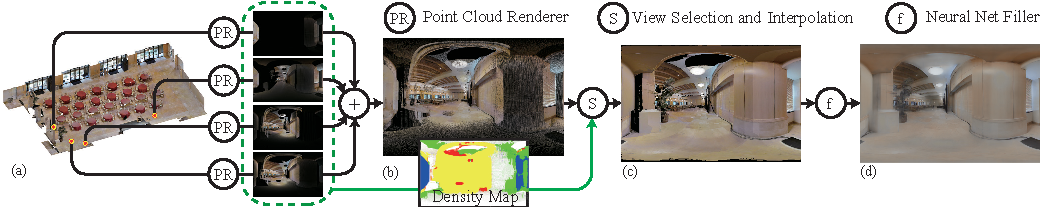
\includegraphics[width=\linewidth]{images/gibson_rendering_pipeline.pdf}
	\caption{The Gibson's rendering pipeline. Image from \cite{gibson}.}
	\label{fig:gibsonrenderingpipeline}
\end{figure}
At first, the given RGB-D panoramas are transformed into point clouds and each pixel is projected from equirectangular coordinates to Cartesian coordinates. For the desired target view $v_j =
(x_j , y_j , z_j , \theta_j, \phi_j, \gamma_j )$, there are chosen the nearest $k$ views in the
scene database, denoted as $v_{j,1}, v_{j,2}, ..., v_{j,k}$. The point cloud of each $v_{j,i}$ coordinate is transformed to $v_j$ coordinate with a rigid body transformation, and the final point cloud is projected onto an equirectangular image (Fig. \ref{fig:gibsonrenderingpipeline}a). Then, the points from all reference panoramas are aggregated to make a single panorama using a locally weighted mixture (Fig. \ref{fig:gibsonrenderingpipeline}b). To do this, the proposed approach calculates the point density for each spatial position (average number of points per pixel) of each panorama. Hence, the points in the aggregated panorama are adaptively selected from all views. Next, the authors perform a bilinear interpolation on the aggregated points of the final panorama
points in one equirectangular image to reduce the empty space between rendered pixels (Fig. \ref{fig:gibsonrenderingpipeline}c). Finally, the method uses a neural network, called $f$ or ``filler'', to fix artifacts and generate a more real-looking image given the output of geometric point cloud rendering (Fig. \ref{fig:gibsonrenderingpipeline}d). This deep model trains a network for making rendered frames look more like real images (forward function) as well as another network that makes real images look like renderings (backward function). The two functions are trained to produce equal outputs. The backward function resembles deployment-time corrective
glasses for the agent, so the authors of \cite{detr} call it \textit{Goggles}.

\subsection{Matterport3D}

In \citeyear{matterport}, \citeauthor{matterport} introduced Matterport3D, a large-scale RGB-D dataset of 90 digitizes real environments. The dataset comprises a set of 194,400 RGB-D images captured in 10,800 panoramas from 90 real-world scenes. It includes both depth and color $360^{\circ} $ panoramas for each viewpoint and provides camera poses that are globally consistent and aligned with a textured surface reconstruction. Furthermore, Matterport3D includes instance-level semantic segmentation into region and object categories.

In the Matterport data acquisition process, an operator captures
a set of panoramas uniformly spaced at approximately 2.5m
throughout the entire walkable floor plan of the environment (Fig. \ref{fig:matterport-panoramas}). It uses a camera system rig with three colors and three depth cameras pointing slightly up, horizontal, and slightly down. At each panorama (acquisition point), the rig rotates around the direction of gravity to
6 distinct orientations, acquiring an HDR photo from each of the 3 RGB cameras for each orientation. The 3 depth cameras acquire data continuously as the rig rotates, which is integrated to synthesize a 1280x1024 depth image aligned
with each color image. The result for each panorama is 18 RGB-D images. 

\begin{figure}[h!]
	\centering
	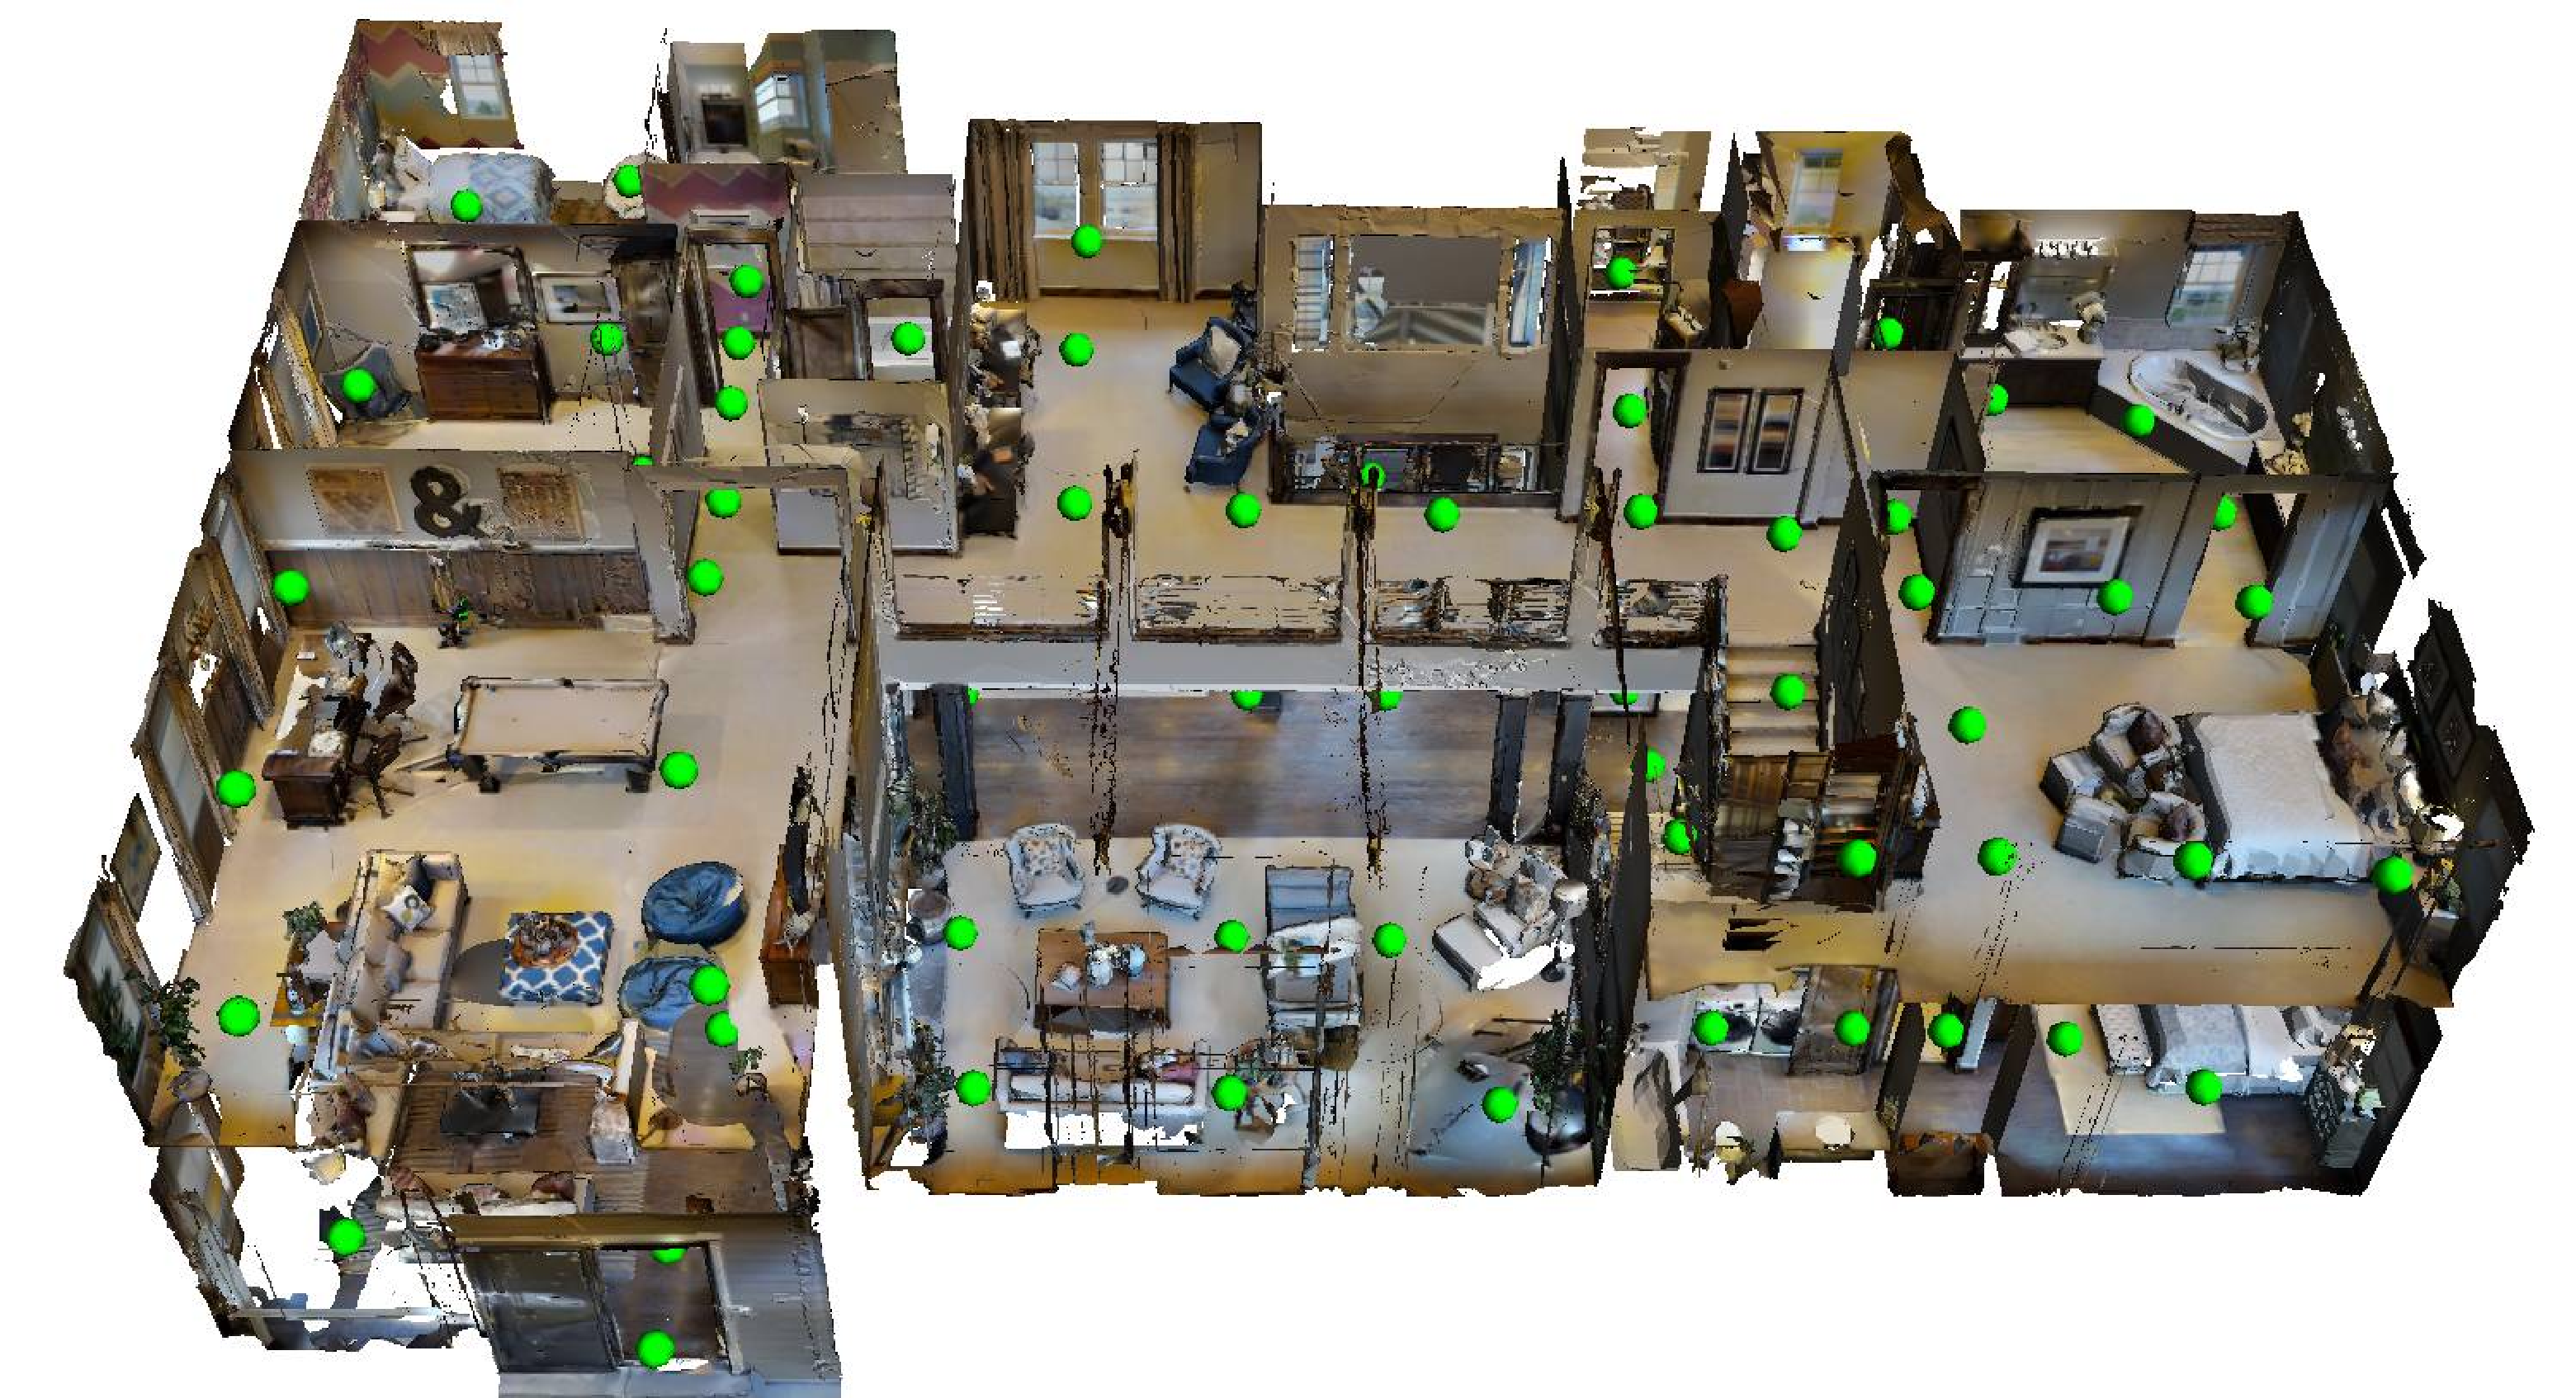
\includegraphics[width=\textwidth]{images/panoramas.pdf}
	\caption{The viewpoints from which panoramas are captured. Image from \cite{matterport}.}
	\label{fig:matterport-panoramas}
\end{figure}

The authors also provide instance-level semantic annotations in 3D. The first step of the annotation process is to break down each building into region components by specifying the 3D spatial extent and semantic category label for
each room-like region. This is done using a simple interactive tool in which the annotator draws a 2D polygon on the floor plans for each region (Fig. \ref{fig:matterport-floor-annotation}). The second step provides an instance and a category level segmentation on objects in each region. Given a 3D mesh of region (Fig. \ref{fig:matterport_object_annotation_1}), the first type of segmentation (instance-level) assigns a different label for each object instance (Fig. \ref{fig:matterport_object_annotation_2}) while the latter (category-level) associates different labels for different object types (Fig. \ref{fig:matterport_object_annotation_3}). To do that, the authors extract a mesh for each region and process it with the crowd-source interface of ScanNet  proposed by \citeauthor{scannet} \cite{scannet}. Using the open-source code provided with ScanNet, the authors of Matterport3D perform surface reconstruction of regions' meshes to ``paint'' triangles to segment and name all object instances
within each region. The 3D segmentations contain a total of 50,811 object
instance annotations divided into 40 objects categories.

\begin{figure}[h!]
	\centering
	\begin{subfigure}[b]{\linewidth}
		\centering
		\begin{subfigure}[b]{0.48\linewidth}
			\centering
			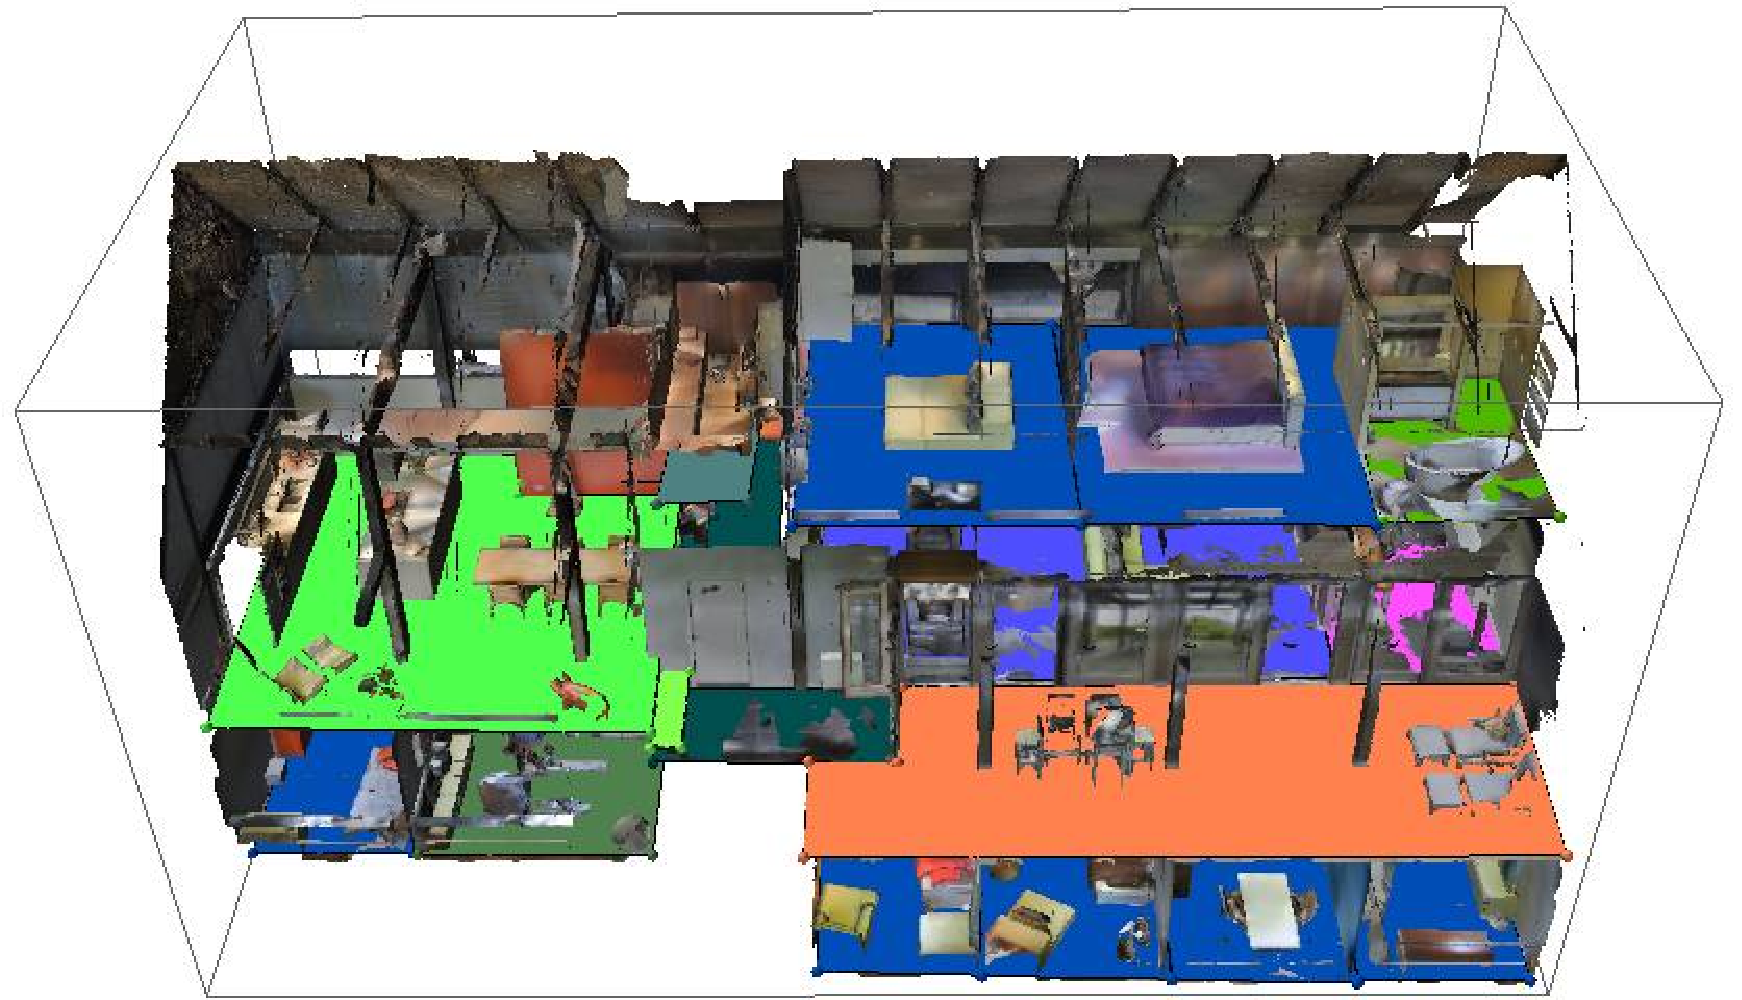
\includegraphics[width=\textwidth]{images/matterport_surfaces_by_label.pdf}
		\end{subfigure}
		\hfil
		\begin{subfigure}[b]{0.48\linewidth}
			\centering
			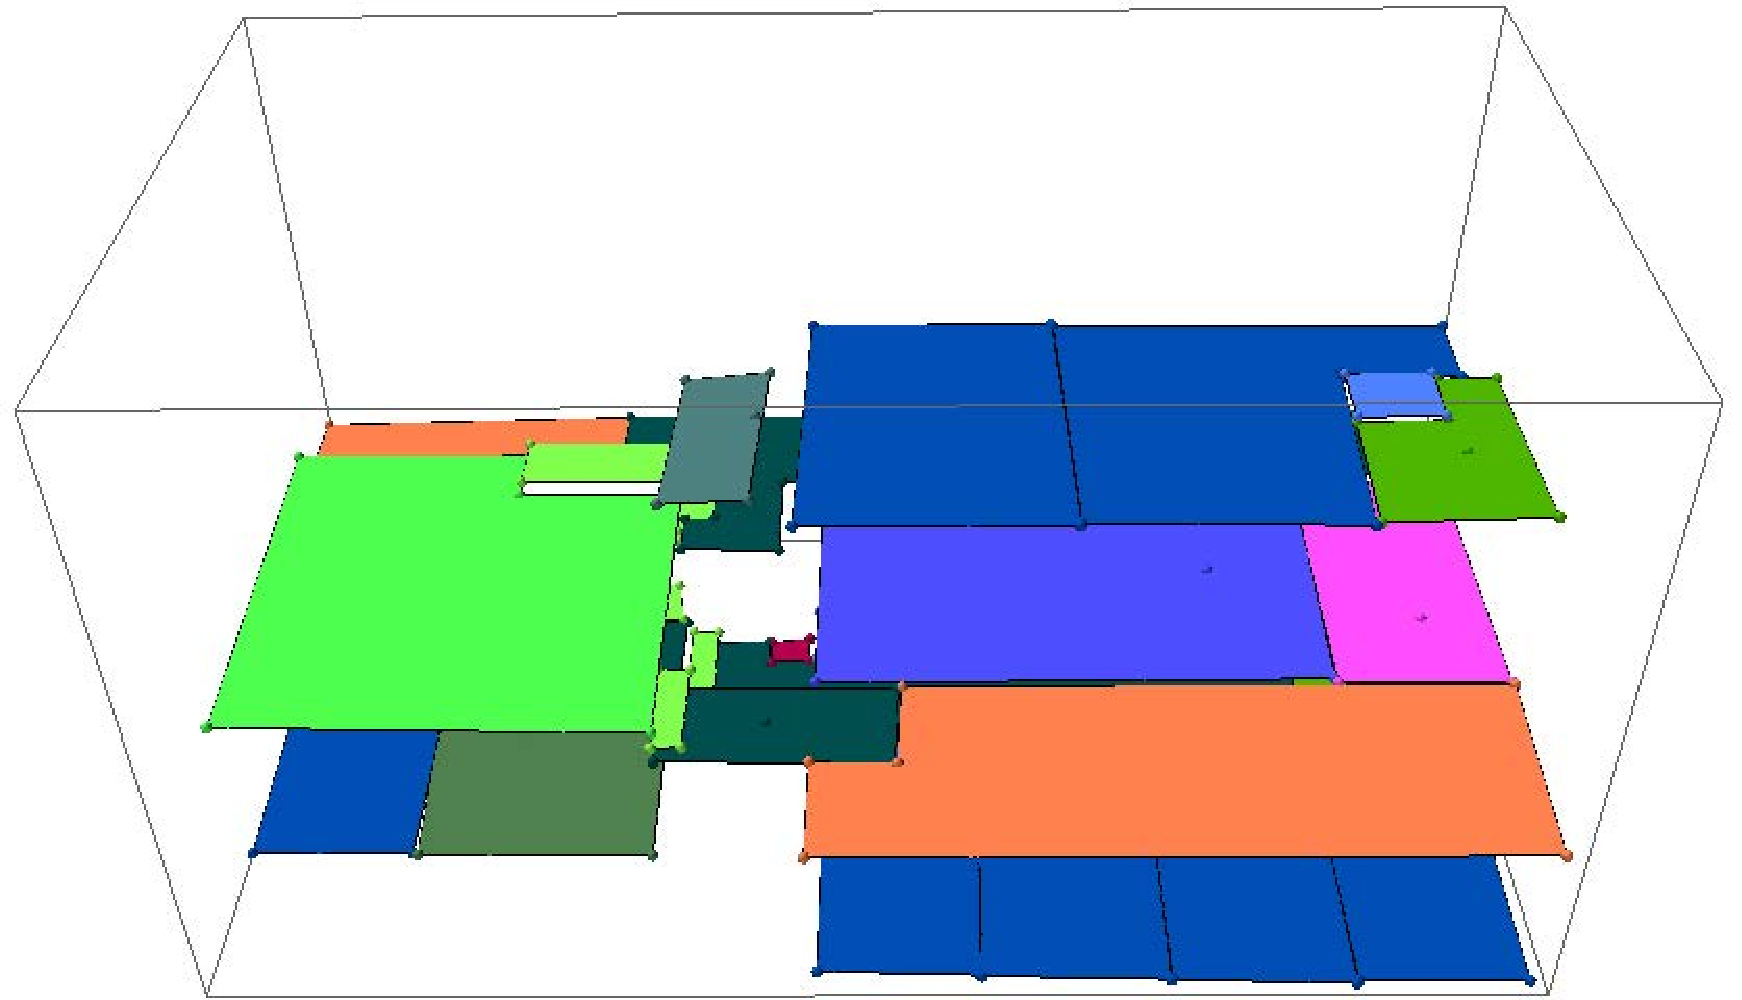
\includegraphics[width=\textwidth]{images/surfaces_by_label.pdf}
			
		\end{subfigure}
	\caption{}
	\label{fig:matterport-floor-annotation}
	\end{subfigure}
	\newline
	\begin{subfigure}[b]{\linewidth}
		\centering
		\begin{subfigure}[b]{0.32\linewidth}
			\centering
			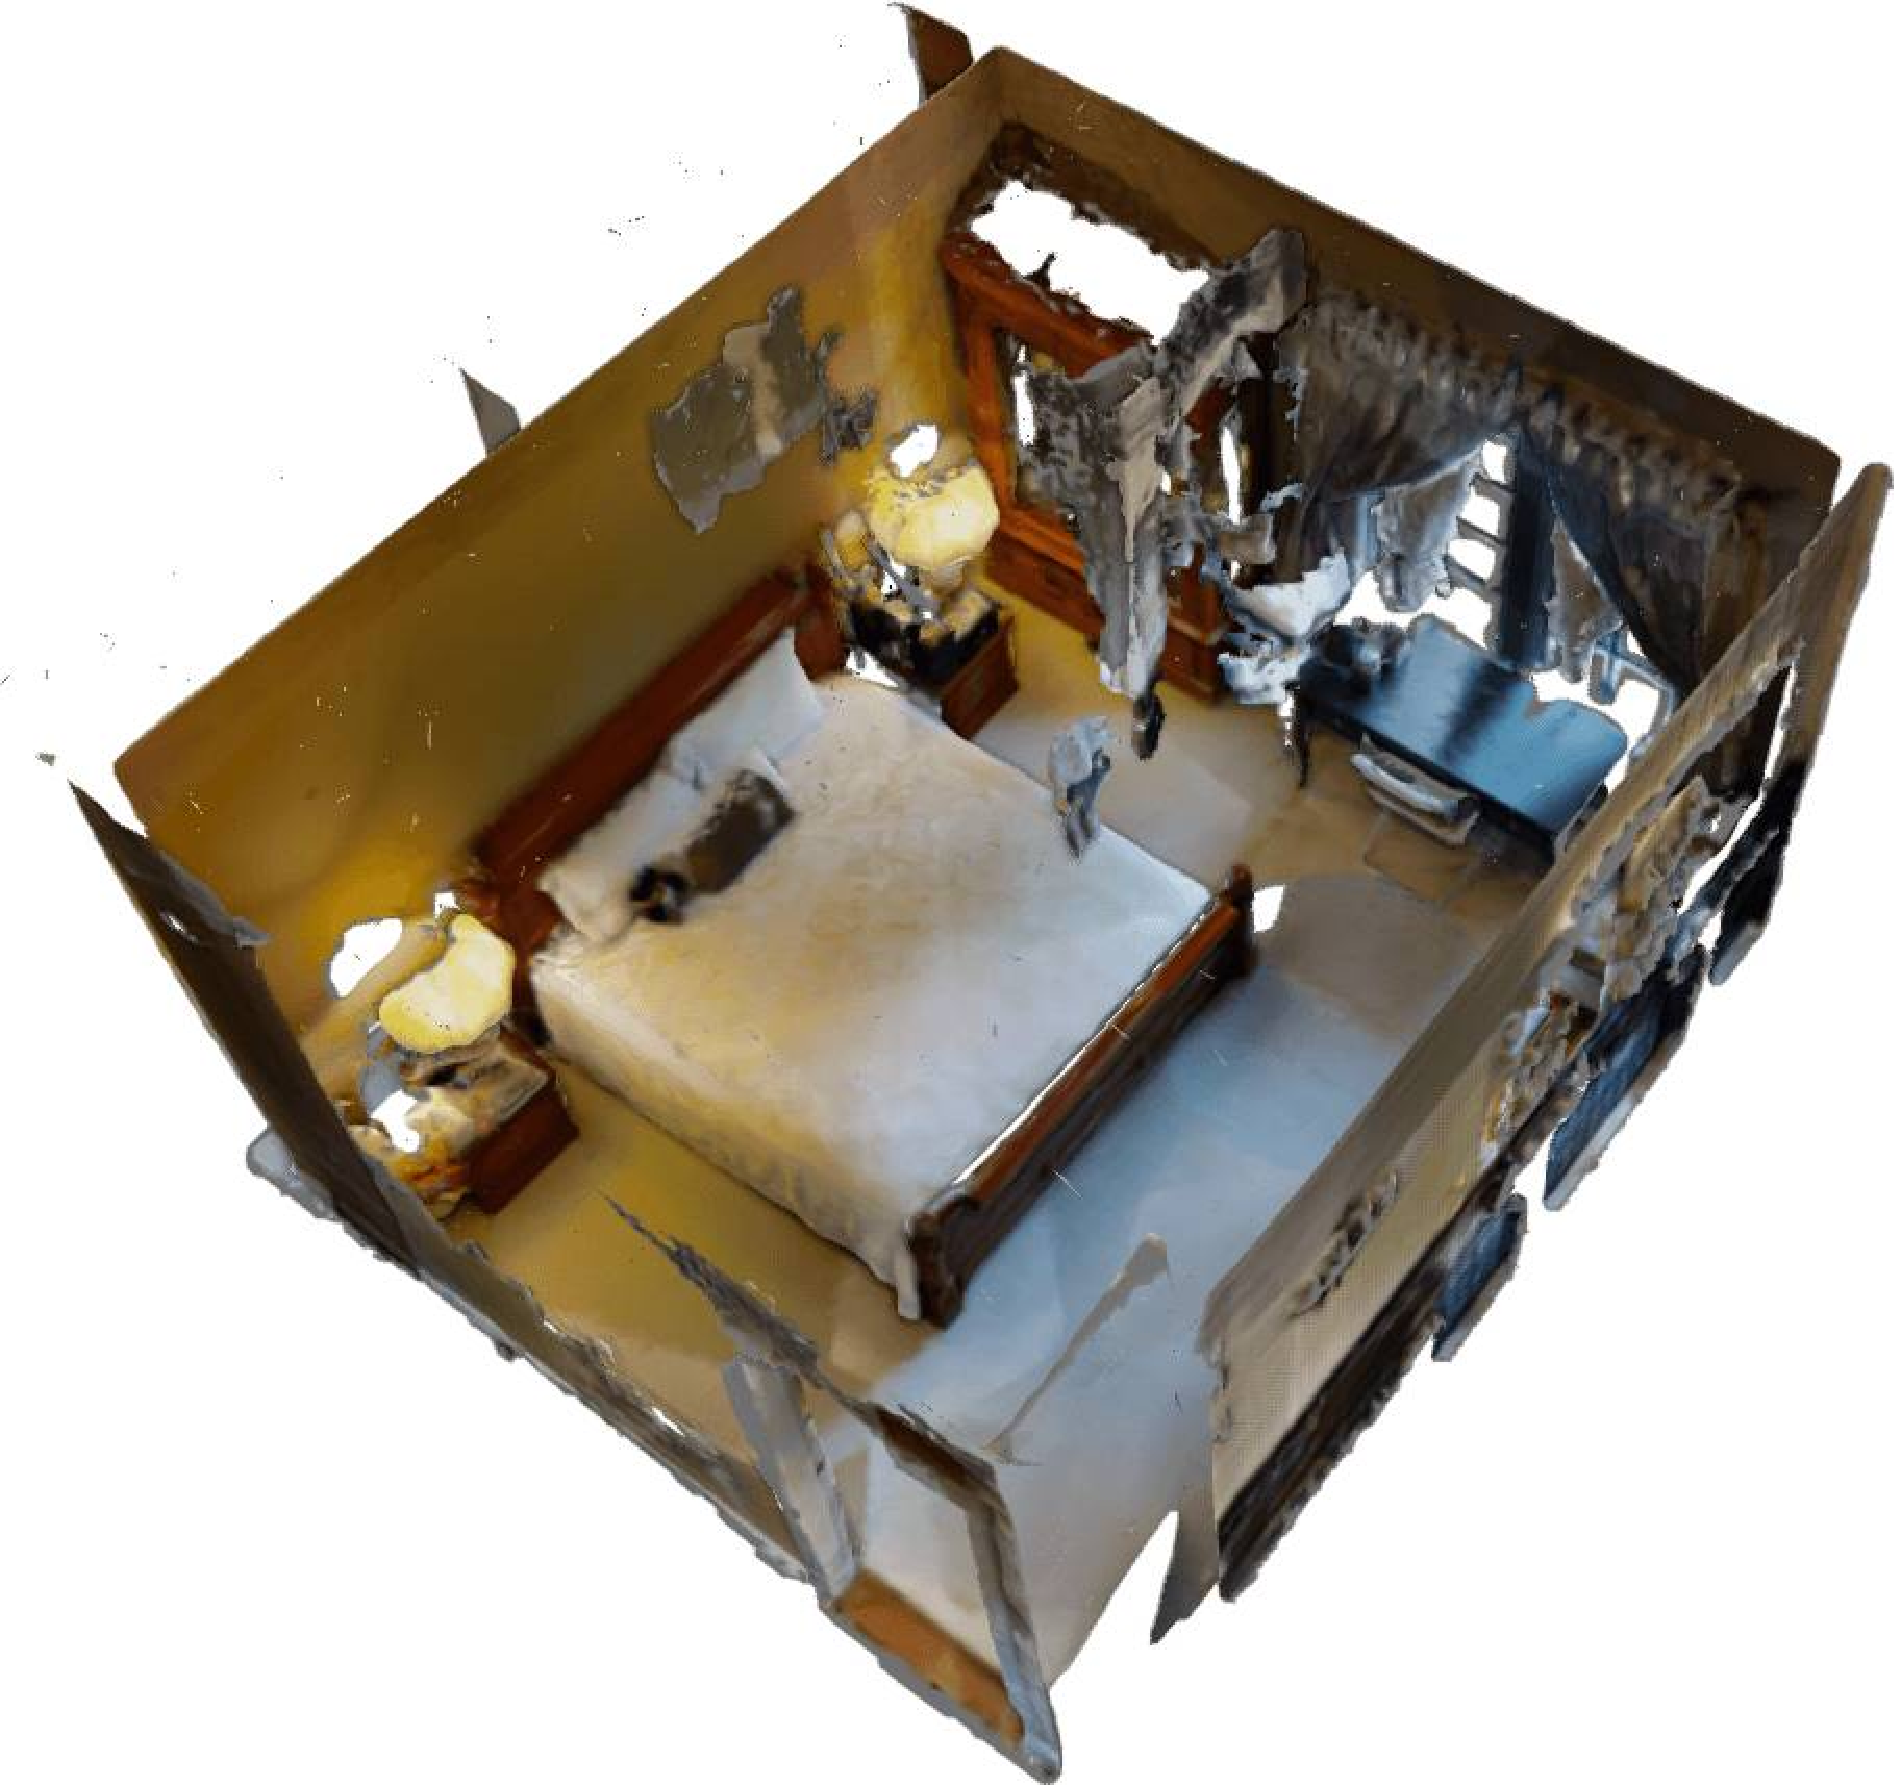
\includegraphics[width=\textwidth]{images/matterport_room22_color.pdf}
			\caption{}
			\label{fig:matterport_object_annotation_1}
		\end{subfigure}
		\hfil
		\begin{subfigure}[b]{0.32\linewidth}
			\centering
			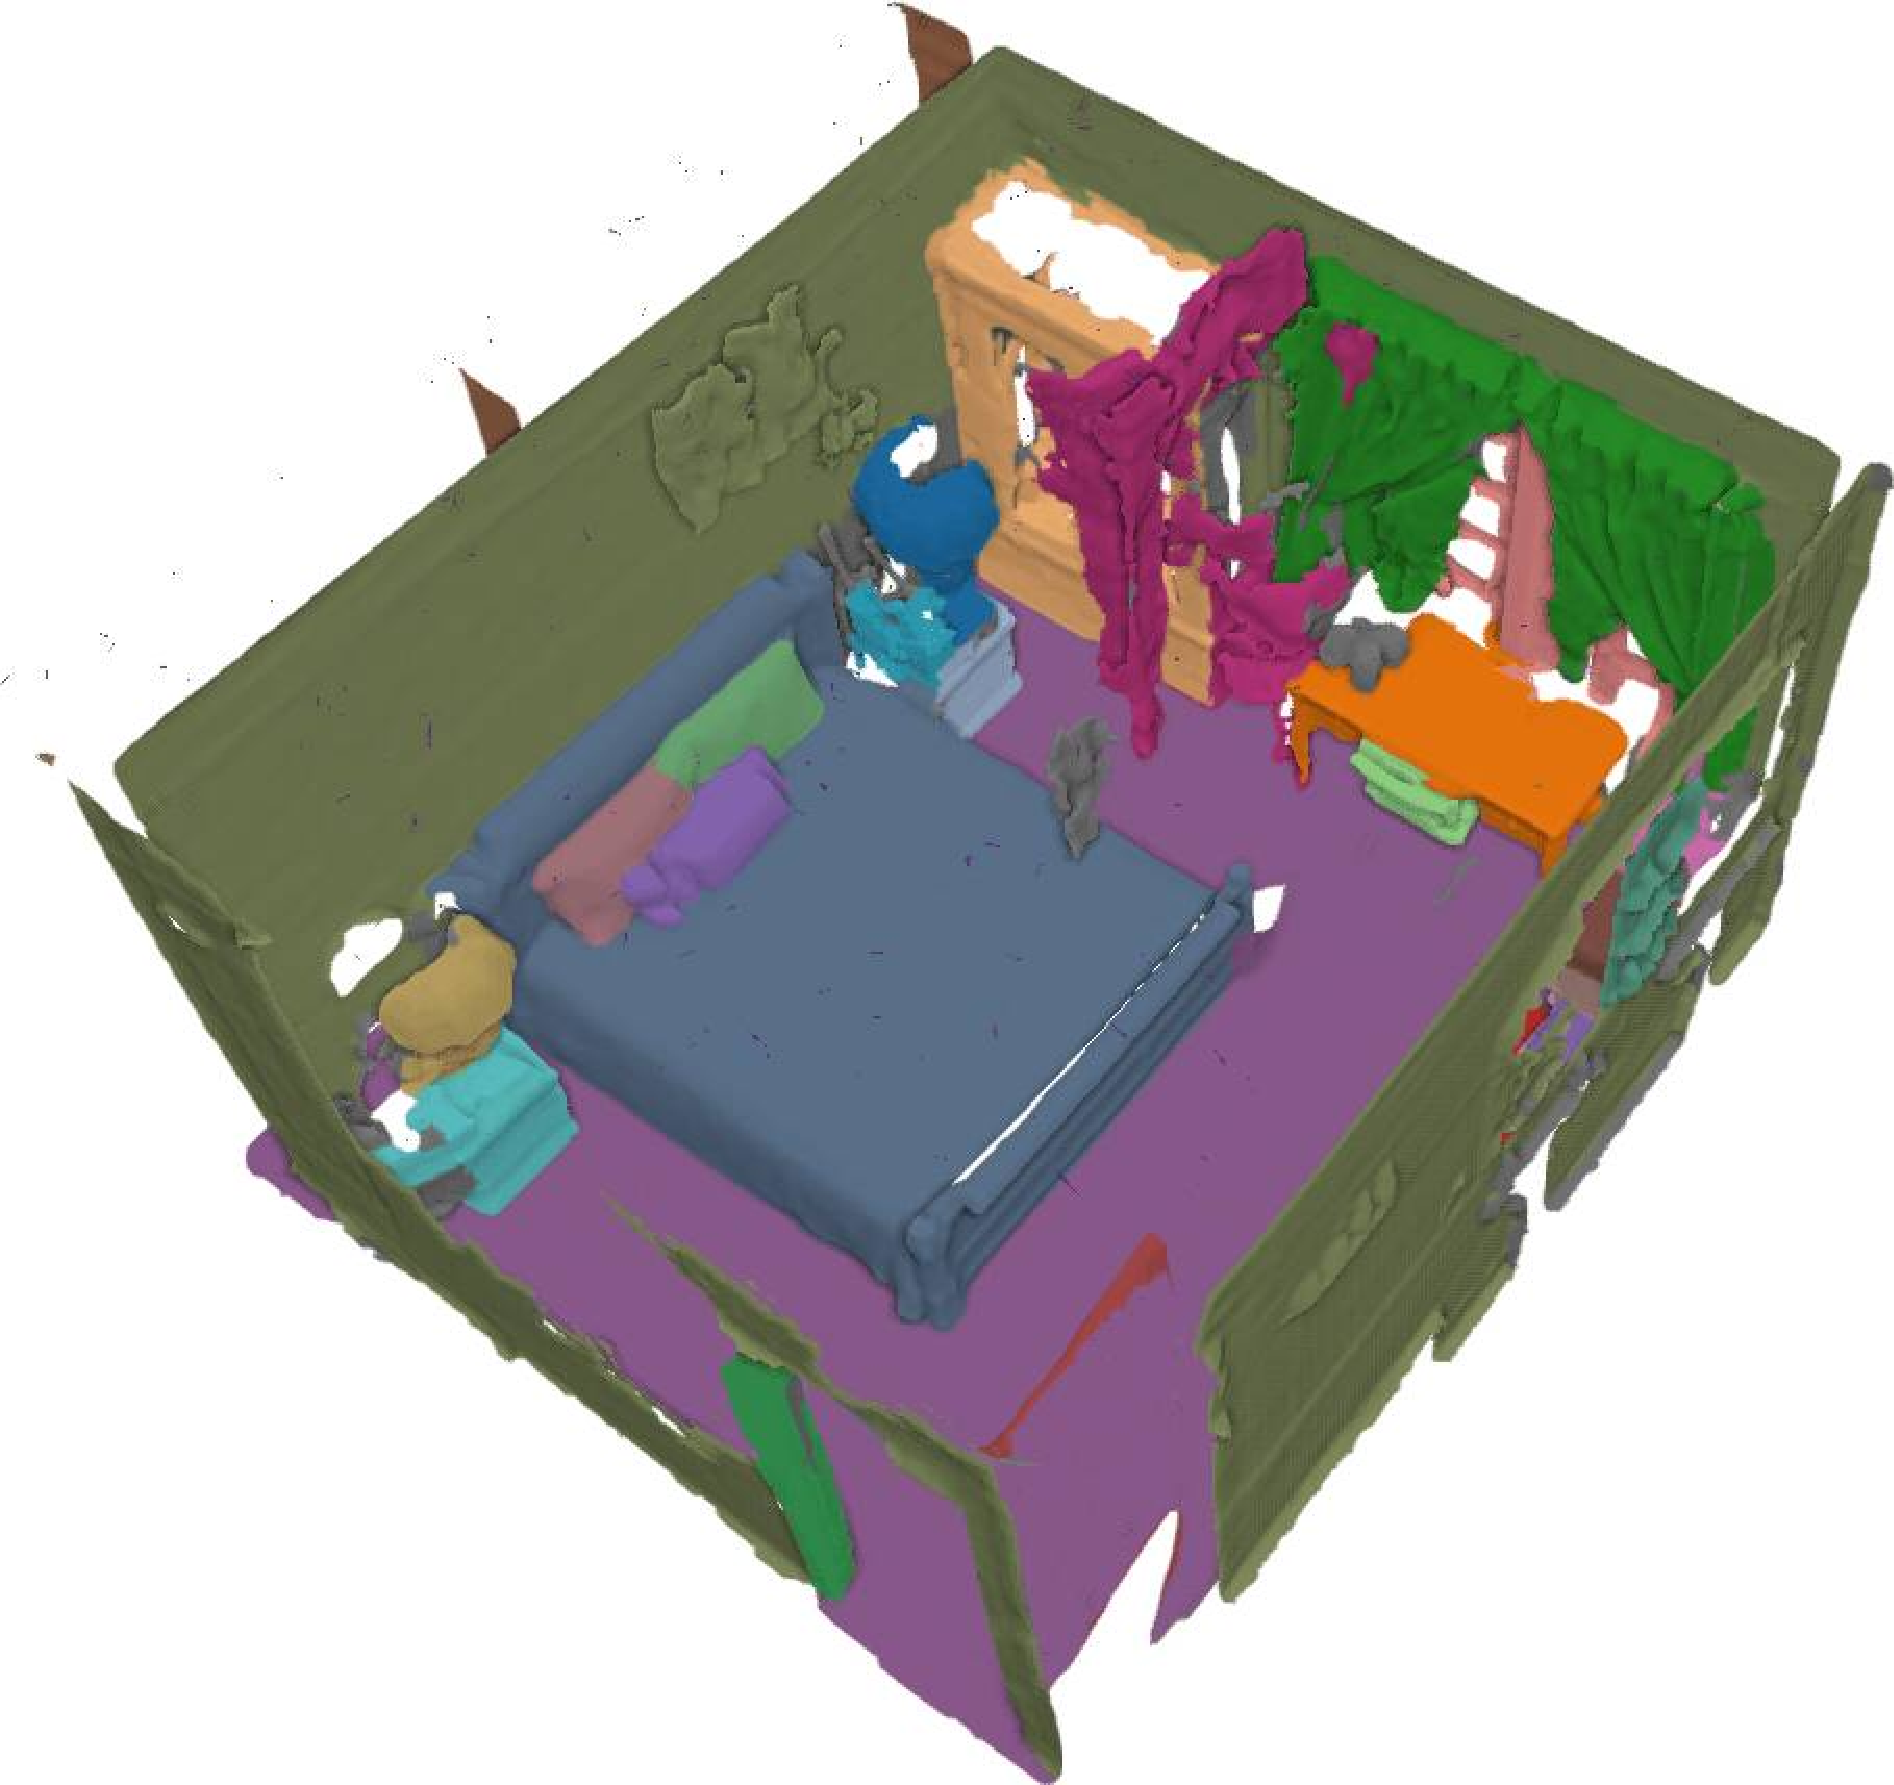
\includegraphics[width=\textwidth]{images/matterport_room22_instances.pdf}
			\caption{}
			\label{fig:matterport_object_annotation_2}
		\end{subfigure}
		\hfil
		\begin{subfigure}[b]{0.32\linewidth}
			\centering
			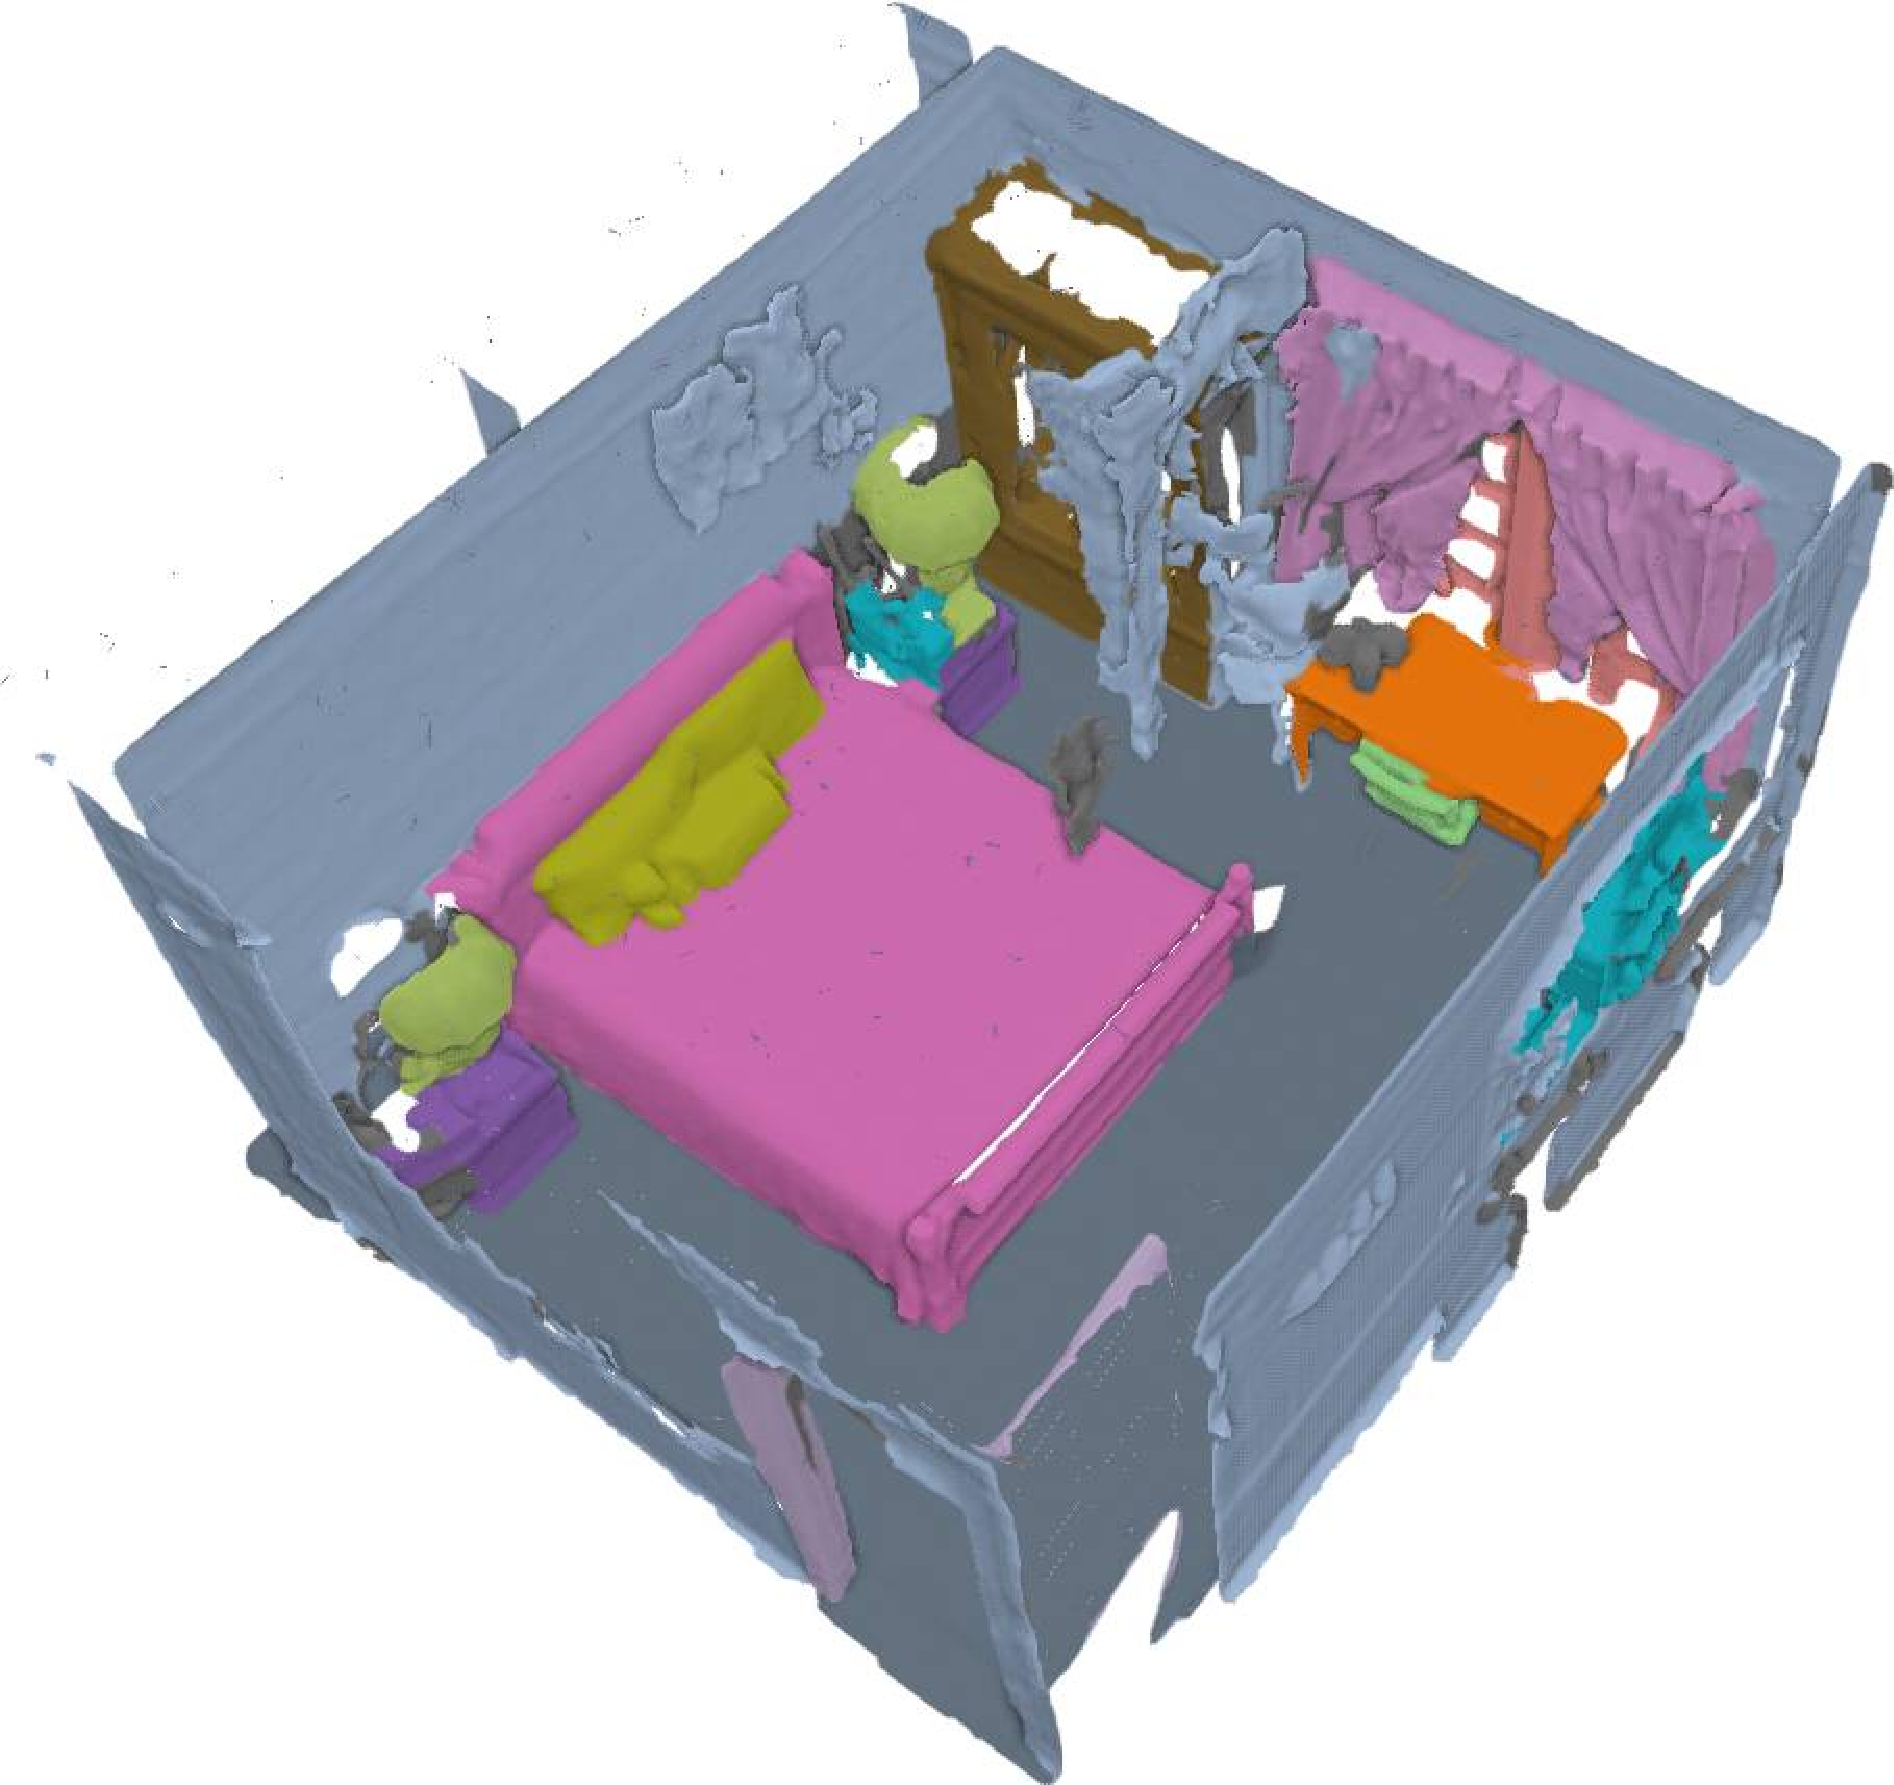
\includegraphics[width=\textwidth]{images/matterport_room22_categories.pdf}
			\caption{}
			\label{fig:matterport_object_annotation_3}
		\end{subfigure}
	\end{subfigure}
	\caption{(a) Region annotation on floor plans. (b, c, d) Instance and category object segmentation of floor plan's region. Images from \cite{matterport}.}
\end{figure}

\subsection{New Gibson Version}
\label{sec:new_gibson_version}

Gibson and Matterport3D are the selected packages to build the dataset to train and evaluate the proposed robotic doors detector. In the first experiments, we argue that these technologies present some problems and limitations that affect an easy and fast data collection procedure. 

A suitable way for acquiring a visual robotic dataset in simulation is to embody a virtual agent which autonomously explores a simulated environment using the standard navigation stack. In this way, the examples captured during its navigation are coherent with a real exploration strategy, reflecting how a real robot would perceive an indoor scene. Unfortunately, this solution is infeasible with the selected technologies. The following paragraphs report the issues related to this technique. 

\paragraph*{Time-Consuming} First of all, this technique is extremely time-consuming. Gibson perfectly simulates the real features of mobile agents (e.g. the speed of movement, the sensors' accuracy, and the physical characteristics). This fact allows us to use the standard navigation stack that is generally provided for well-known mobile robots (e.g. Turtlebot2 \cite{turtlebot2}, Turtlebot3 \cite{turtlebot3}, or Husky car \cite{husky}). Despite this, the real-time simulation provided by Gibson makes the data acquisition extremely slow, especially for large environments.  Furthermore, the dataset would be suitable for multiple robots with different navigation packages and camera heights. This fact implies performing multiple runs in the same environments with different agents, further extending the acquisition time. Due to the fact that navigation is a challenging task, an autonomous agent can crash into an obstacle or iterate the same actions due to a software issue. In simulated environments, fixing robot failures is often infeasible, making the runs useless. 

\paragraph*{Experiment Repeatability} Another issue is related to the exploration, which can be performed through different strategies (such as frontier-based exploration \cite{frontierexploration}) that do not guarantee the experiments' repeatability. In different runs, the robot can follow different paths and the exploration time can vary a lot. In this way, the dataset is heavily dependent on the chosen exploration strategy.

\paragraph*{Inaccuracy of the Worlds' Dataset} While the issues just reported can be solved using appropriate techniques, the problem related to the Matterport3D dataset makes completely infeasible to perform data collection using Gibson ``as is''. The physical structure of the Matterport's environments is encoded in 3D polygonal meshes. A polygon mesh is a collection of vertices, edges, and faces that defines the shape of a polyhedral object. These meshes are extremely cluttered and noisy. The furniture models are malformed and incomplete, e.g. a table can be composed of the horizontal plan omitting one or more legs (Fig. \ref{fig:matterport_issues_meshes_furniture}), or some faces are disconnected from the principal object mesh. Furthermore, the walls often present holes at windows, mirrors, or other undefined locations (Fig. \ref{fig:matterport_issues_hole}). These artifacts affect the robot perception, making autonomous navigation impossible. Another important aspect concerns the floor plans' surfaces, that are extremely irregular. They are composed of a series of triangles but the vertexes are not perfectly aligned (Fig. \ref{fig:matterport_issues_floor_plan}). This further complicates the robot navigation, which often crashes over floor irregularities.

\begin{figure}[h!]
	\centering
	\begin{subfigure}[b]{0.32\linewidth}
		\centering
		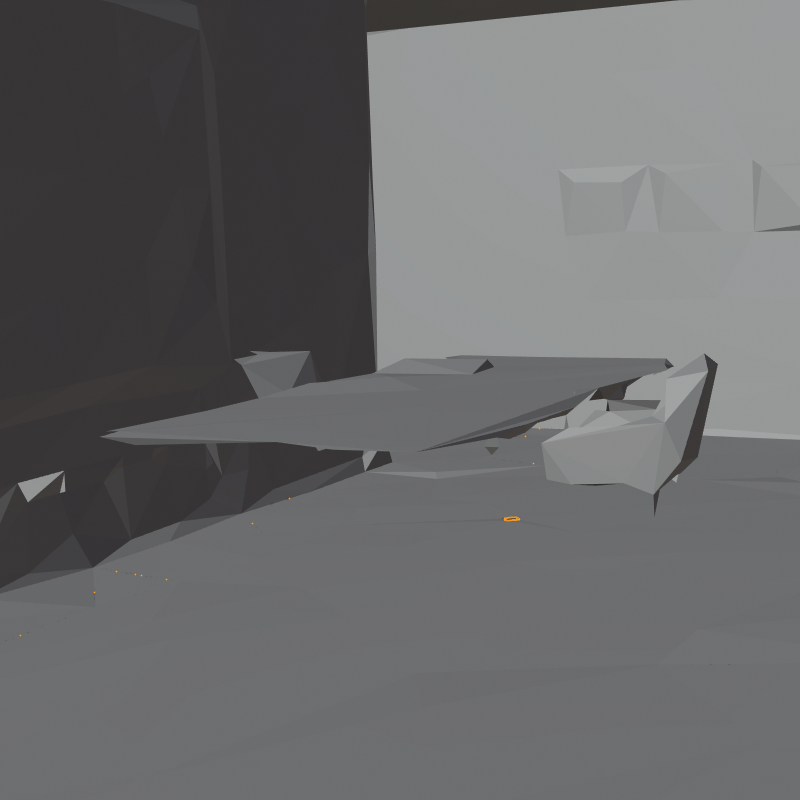
\includegraphics[width=\textwidth]{images/table.png}
		\caption{}
		\label{fig:matterport_issues_meshes_furniture}
	\end{subfigure}
	\hfil
	\begin{subfigure}[b]{0.32\linewidth}
		\centering
		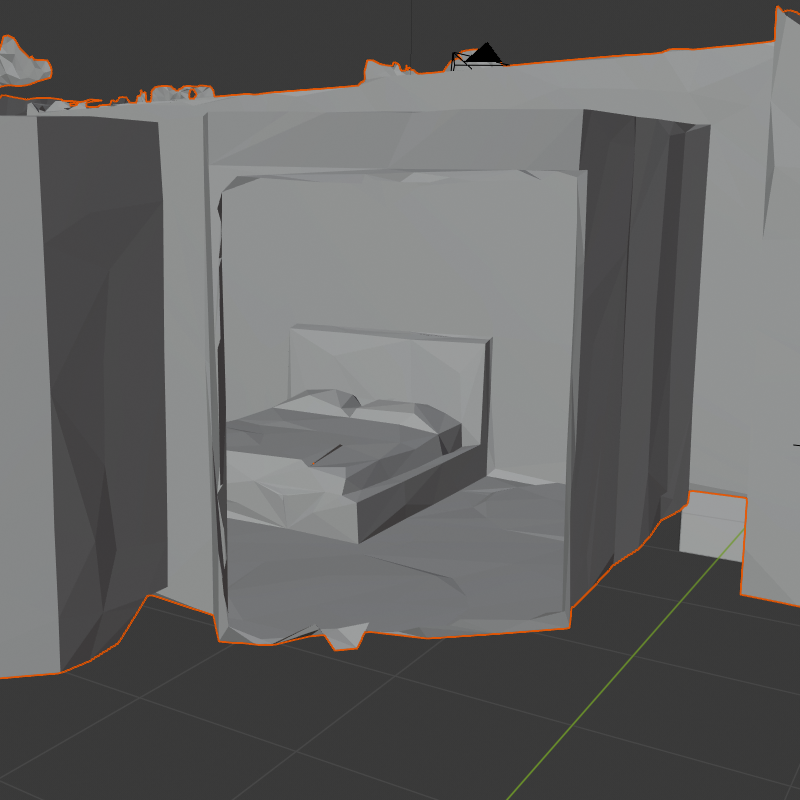
\includegraphics[width=\textwidth]{images/holes.png}
		\caption{}
		\label{fig:matterport_issues_hole}
	\end{subfigure}
	\hfil
	\begin{subfigure}[b]{0.32\linewidth}
		\centering
		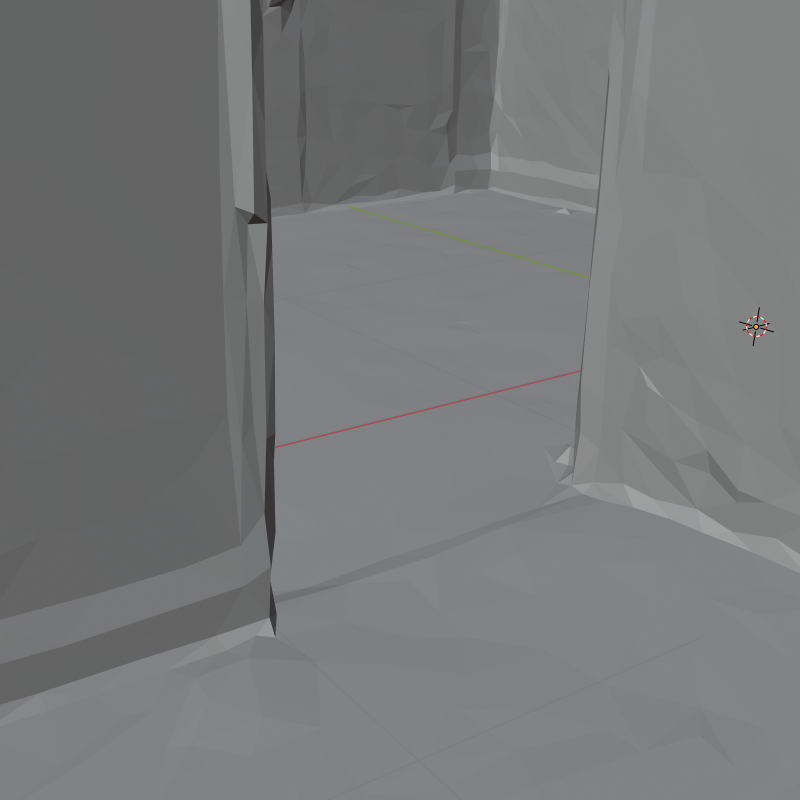
\includegraphics[width=\textwidth]{images/floor_plan_irregularity.png}
		\caption{}
		\label{fig:matterport_issues_floor_plan}
	\end{subfigure}
	\caption{Matterport3D mesh malformations. (a) A suspended table and chair. (b) A holes in a bedroom. (c) Floor plan irregularities.}
\end{figure}


To overcome these difficulties, we provide an upgraded version of Gibson available on Github\footnote{The code of the new Gibson version: \url{https://github.com/micheleantonazzi/GibsonEnv}.}. We developed a new simulation mechanism without any physical constraints: gravity and collision detection are removed. Inside this stage, the robot can not move autonomously using motors, but the user can set an absolute position and orientation in which the robot must be located at each instant. In other words, we implement a less realistic simulation mechanism in which a robot can both instantly teleport in any location and traverse obstacles. In this way, the user can perform data acquisition in batch without any failure. The robot does not crash over the floor's irregularities (that are due to artifacts), does not go out of the mesh, and can autonomously traverse multiple floors without dealing with architectural barriers (such as stairs or elevators).

The new version of Gibson we released implements further improvements. First of all, we resolve some building errors (that occurs especially in Ubuntu 20.04), and automatize the compile procedure, implementing it inside the \textsf{setup.py} file. In this way, with the simple command \textsf{pip install gibson}, the simulation environment is compiled and installed. The necessary dependencies have been added as Git sub-modules. In this way, they are automatically downloaded and compiled, simplifying the dependencies management. Then, we developed a new and more efficient module to manage Gibson's assets, such as the neural network's weights, the virtualized agents, or the worlds dataset. We also offer a command-line interface to automatically download and extract the assets files from the links provided by the authors. To use it, the user can type three different commands (after Gibson's installation) in a console terminal: \textsf{gibson-set-assets-path} for specifying the assets' folder, \textsf{gibson-download-dataset} to download the provided worlds dataset, and \textsf{gibson-download-assets-core} to retrieve the remaining assets files. Finally, we provide a compiled version of Gibson available on PyPI\footnote{The compiled version of Gibson: \url{https://pypi.org/project/gibson/}.} following the manylinux standard\footnote{The manylinux repository: \url{https://github.com/pypa/manylinux}.}. We offers also a utility package, called \textit{gibson-env-utilities}\footnote{The gibson-env-utilities source code: \url{https://github.com/micheleantonazzi/gibson-env-utilities}.}, to facilitate the usage of Gibson. It automatizes the launch of simulation runs, by offering a class that automatically creates the Gibson configuration file in which the parameters of the run are specified. Furthermore, \textit{gibson-env-utilities} provides a mechanism to store and retrieve the metadata related to Gibson's scenes. This metadata includes the environment name, the belonging dataset (Matterport3D \cite{matterport} or Stanford-2D-3D \cite{stanford2d3d}) a boolean value that indicates if the environment is semantically annotated, and the number of floors. In addition, for each floor is provided the floor's height and a valid position on such a floor in which the robot can be placed.


\section{Pose Estimator}
\label{sec:pose_estimator}
To acquire a valid vision dataset, we need to determine the valid positions in which the robot can be placed: it must be in free space inside the building perimeter and not colliding with obstacles (walls, floors, or furniture). Furthermore, the samples must be collected in locations consistent with a possible exploration strategy followed by a mobile robot. Typically, a robot walks away from obstacles and chooses the shortest path for moving between different areas. To address these requirements, we developed a method called Pose Estimator, which is based on the work proposed by \citeauthor{repeatabilityslamarxiv} in \cite{repeatabilityslamarxiv, repeatabilityslam}.

  is the component that extracts plausible positions for an autonomous agent from which collect the dataset. This tool performs the computation of the Voronoi graph over the 2D occupancy grid map \cite{cuupancygridfirst} of a floor plan and chooses the positions by sub-sampling this graph. The following paragraphs describe the procedures performed by this module, which is implemented in the \textit{gibson-env-utilities} package.



\paragraph*{Extract the 2D Occupancy Grid} The first step concerns the computation of a 2D occupancy grid map (Fig. \ref{fig:pose_estimator_occupancy_grid}) of a floor starting from a 3D mesh (Fig. \ref{fig:pose_estimator_3dmesh}). Each environment of Matterport3D is modeled by a 3D Wavefront file (with \textit{.obj} extension) that stores the position of each vertex and the faces that compose each polygon. The 3D model of an environment is rendered, using a software like Blender\footnote{The Blender's web page: \url{https://www.blender.org/}.}, to estimate the average height of the points that compose the selected floor plan. Then, the method performs multiple cross-sections of the 3D mesh with parallel planes, starting from a few centimeters over the floor. The 2D cross-sections, that detect obstacles at multiple heights, are aggregated and projected in a 2D image. Finally, this image is manually fixed to fill the shortcomings due to mesh inaccuracies or to remove artifacts produced by the cross-section. In addition, it is particularly important that, during this step, the opened contours in the image are closed. This final 2D image (Fig. \ref{fig:pose_estimator_occupancy_grid}) stores the occupancy grid map of a floor plan, where each pixel represents a sub-portion of the environment and contains the probability that it is occupied by an obstacle. Together with the image map, important metadata are also saved, in order to enable conversion operations between map and simulation coordinates. The metadata includes the map's origin (in pixels) and the scale, which specifies how many meters correspond to a pixel.

These operations are implemented in the \textsf{GibsonAssetsUtilities} class of \textit{gibson-env-utilities} package. In particular, \textsf{load\_obj} method loads the Wavefront file while \textsf{create\_floor\_map} extract the floor map and the relative metadata, saving them to the disk. The mesh file loading and the computation of multiple cross-sections are performed using Trimesh\footnote{The Trimesh source code: \url{https://github.com/mikedh/trimesh}.}, a pure Python library for loading and elaborating triangular meshes. The final image is rendered using Matplotlib\footnote{The Matplotlib web site: \url{https://matplotlib.org/}.}, a comprehensive library for creating static, animated, and interactive visualizations in Python. 

\begin{figure}[h!]
	\centering
	\begin{subfigure}[b]{0.49\linewidth}
		\centering
		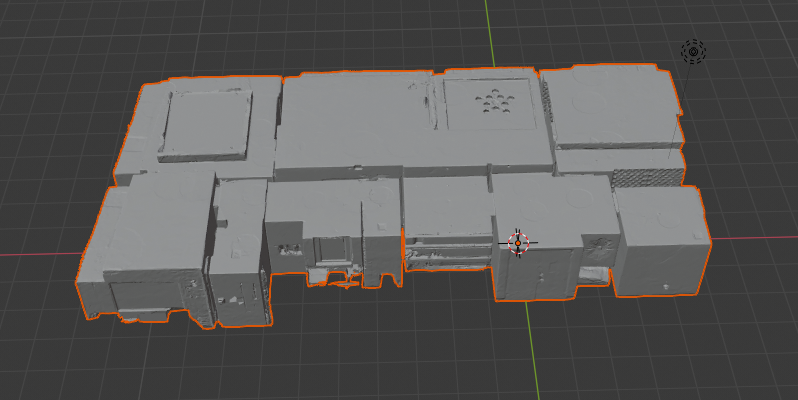
\includegraphics[width=\textwidth]{images/pose_estimator_3Dmesh.png}
		\caption{}
		\label{fig:pose_estimator_3dmesh}
	\end{subfigure}
	\hfil
	\begin{subfigure}[b]{0.49\linewidth}
		\centering
		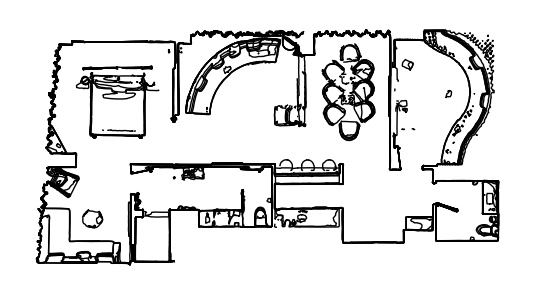
\includegraphics[width=\textwidth]{images/pose_estimator_1.png}
		\caption{}
		\label{fig:pose_estimator_occupancy_grid}
	\end{subfigure}
	\caption{The computation of the 2D occupancy grid map (right) from the 3D mesh (left) of an environment.}
\end{figure}

\newpage

\paragraph*{Compute the Voronoi Bitmap} This step aims to extract the Voronoi bitmap graph from the 2D occupancy grid of a floor (Fig. \ref{fig:pose_estimator_1}). In order to do this, Pose Estimator processes the occupancy grid map, stored in a \textsf{png} image, using OpenCV\footnote{The OpenCV home page \url{https://opencv.org/}.}: a library of programming functions mainly aimed at real-time computer vision. At first, the image is thresholded to obtain a more uniform mask which indicates the free and occupied location. To do this, the module uses the OpenCV's \textsf{threshold} method, which suppresses (leads to zero) all pixels with a color value less than 250. Then, this optimized occupancy grid is eroded and dilated (through the \textsf{erode} and \textsf{dilate} methods of OpenCV) using a $3 \times 3$ kernel to reduce the noise. Now, the method finds the contours (using the OpenCV \textsf{findContours} method) in the smoothed image to identify the boundaries in which the robot can move. The methods return all the contours in the image without any approximation organized in a tree structure, thanks to the \textsf{CHAIN\_APPROX\_NONE} and \textsf{RETR\_TREE} flags respectively. The longest contour is assumed to be the floor's perimeter. The area outside the floor's outline and all its internal contours (that represent the furniture) are black-filled: the resulting image (Fig. \ref{fig:pose_estimator_filled}) highlights in white the free area in which the robot can move. Now, the Voronoi diagram is calculated using the Delaunay triangulation \cite{delaunayproof} (implemented by the OpenCV class \textsf{SubDiv2D}) using all the points belonging to the identified contours.  The Voronoi facets, obtained with \textsf{getVoronoiFacetList} method of the \textsf{SubDiv2D} instance, are drawn in a new image, reporting only the segments inside the white area of the black filled image. The drawn segments compose the bitmap of the Voronoi graph (Fig. \ref{fig:pose_estimator_voronoi_bitmap}) computed over a floor occupancy grid map. As shown by (Fig. \ref{fig:pose_estimator_voronoi_bitmap_map}), the Voronoi bitmap does not exceed the floor's contours and does not overlap furniture. 

\begin{figure}[h!]
	\centering
	\begin{subfigure}[b]{0.49\linewidth}
		\centering
		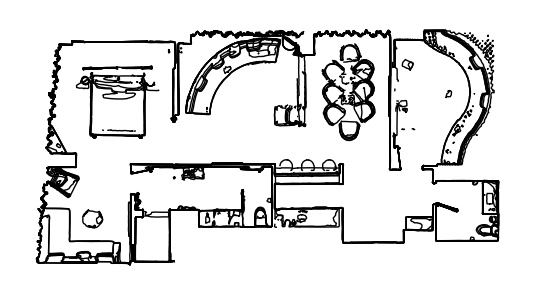
\includegraphics[width=\textwidth]{images/pose_estimator_1.png}
		\caption{}
		\label{fig:pose_estimator_1}
	\end{subfigure}
	\hfil
	\begin{subfigure}[b]{0.49\linewidth}
		\centering
		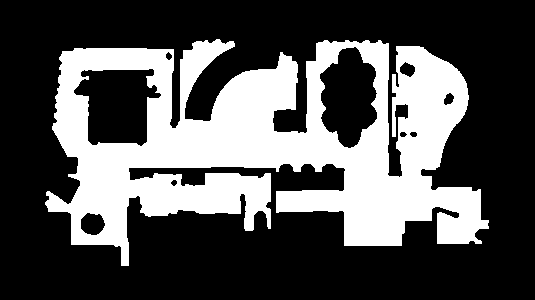
\includegraphics[width=\textwidth]{images/pose_estimator_filled_contours.png}
		\caption{}
		\label{fig:pose_estimator_filled}
	\end{subfigure}
	\newline
	\begin{subfigure}[b]{0.49\linewidth}
		\centering
		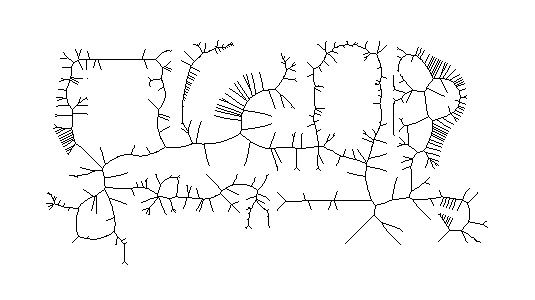
\includegraphics[width=\textwidth]{images/pose_estimator_bitmap_voronoi.png}
		\caption{}
		\label{fig:pose_estimator_voronoi_bitmap}
	\end{subfigure}
	\hfil
	\begin{subfigure}[b]{0.49\linewidth}
		\centering
		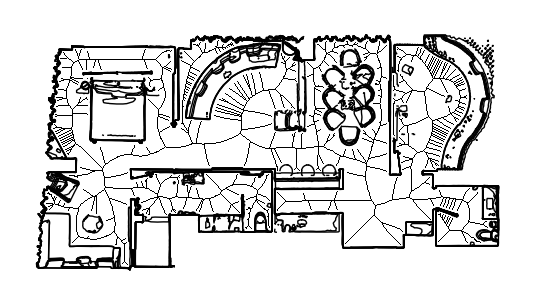
\includegraphics[width=\textwidth]{images/pose_estimator_bitmap_map.png}
		\caption{}
		\label{fig:pose_estimator_voronoi_bitmap_map}
	\end{subfigure}
	\caption{The computation of the Voronoi bitmap. In a 2D occupancy grid map of a floor (a), the free space is isolated in white (b), and the Voronoi graph is generated through Delaunay triangulation (c, d).}
	\label{fig:pose_estimator}
\end{figure}

\newpage

\paragraph*{Voronoi Graph Pruning and Digitization} The last step aims to extracts the graph described by the Voronoi bitmap and prune it to remove the spurious sidelines. More formally, we represent this graph as $G = (V, E)$, where the vertices are the black pixels in the Voronoi bitmap and the edges (that define symmetric relations between vertices) are implicitly stored inside nodes (each nodes specify its neighbors). 

To build a graph starting from a Voronoi bitmap (Fig. \ref{fig:pose_estimator_bitmap}), we parse the image to build an instance node for each black pixel in the bitmap, adding them to a graph object. The \textsf{node} and \textsf{graph} classes are implemented in a file called \textsf{utilities/graph.py} of \textit{gibson-env-utilities} package. Each node is described by its coordinates in the image expressed in pixel. Then, the method proceeds with the identification of adjacent nodes that compose the graph. For each node, the approach searches the neighboring nodes inside the $3 \times 3$ pixels area centered in the current node's image coordinates. If a pixel in such area belongs to the Voronoi bitmap, the correspondent node is added to the neighbors' list of the current node and vice-versa, creating a double connection between them. The graph can be composed of multiple sub-components disconnected from each other. In other words, the initial graph $G = (N, V)$ is partitioned in multiple sub-graphs $g_1, g_2, ..., g_n$, where each sub-graphs $g_i$ is a connected component formed by a sub-set of nodes $g_i \in N \setminus \bigcup_{y=1}^{n} g_{y}, \mid y  \neq i$. Initially, the method preserves all the sub-graphs. 

The algorithm proceeds pruning the spurious sidelines. To do this, the method parses each sub-graph to recursively remove each node with a single neighbor. In other words, when the recursive function encounters the end of a sideline, it deletes the last node and consequently removes the others until the line beginning, where there is a crossroads. A plot of the pruned graphs is shown in Fig. \ref{fig:pose_estimator_pruned_lines}. 

Then the graph is printed in a new Voronoi bitmap to be further refined. The new image is subject to a dilation operation immediately followed by an image skeletonization. These two operations are necessary to obtain a bitmap Voronoi graph as clean and uniform as possible. The images dilation is performed through the OpenCV's \textsf{dilate} method, applied with a $3 \times 3$ kernel, while the skeletonization is implemented by a function provided by scikit-image\footnote{The scikit-image website: \url{https://scikit-image.org/}.}, a library designed for image processing.
Since the skeletonization function requires a binary image expressed in $[0, 1]$ range, the Voronoi bitmap is converted in a binary image encoded in such interval. After this operation, the image is re-converted in the OpenCV's format, in which pixels can assume a value between 0 and 255. The skeletonized Voronoi bitmap is shown in Fig. \ref{fig:pose_estimator_skelethon}. 

Finally, the last pruned and skeletonized Voronoi bitmap is re-parsed to build a new and more refined Voronoi graph, using the same procedure previously explained. A representation of the final graph can be seen in Fig. \ref{fig:pose_estimator_skelethon_map}. 
 
\begin{figure}[h!]
	\centering
	\begin{subfigure}[b]{0.49\linewidth}
		\centering
		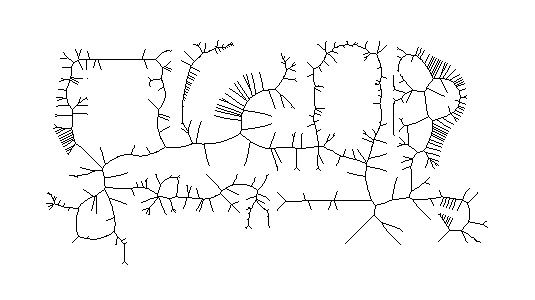
\includegraphics[width=\textwidth]{images/pose_estimator_bitmap_voronoi.png}
		\caption{}
		\label{fig:pose_estimator_bitmap}
	\end{subfigure}
	\hfil
	\begin{subfigure}[b]{0.49\linewidth}
		\centering
		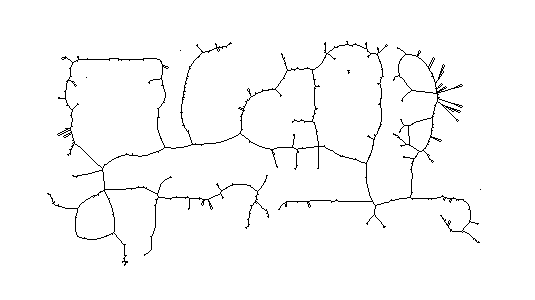
\includegraphics[width=\textwidth]{images/pose_estimator_pruned_lines.png}
		\caption{}
		\label{fig:pose_estimator_pruned_lines}
	\end{subfigure}
	\newline
	\begin{subfigure}[b]{0.49\linewidth}
		\centering
		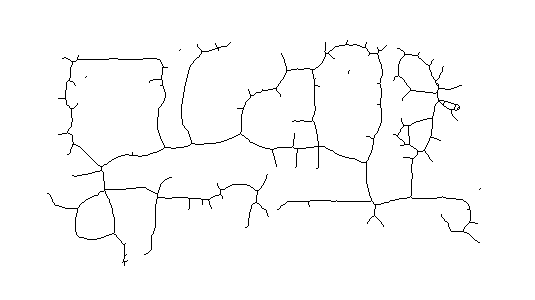
\includegraphics[width=\textwidth]{images/pose_estimator_skelethonization.png}
		\caption{}
		\label{fig:pose_estimator_skelethon}
	\end{subfigure}
	\hfil
	\begin{subfigure}[b]{0.49\linewidth}
		\centering
		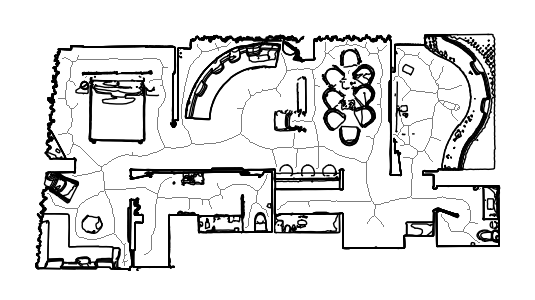
\includegraphics[width=\textwidth]{images/pose_estimator_skelethon_map.png}
		\caption{}
		\label{fig:pose_estimator_skelethon_map}
	\end{subfigure}
	\caption{The steps for pruning the Voronoi bitmap. The initial image (a) is digitized and pruned using a recursive function to remove the side lines (b). Then, the Voronoi graph is printed in a new image and skeletonized using scikit-image function (c, d). }
\end{figure}

\paragraph*{Voronoi Graph Sub-Sampling} The last step performed by Pose Estimator concerns sub-sampling the Voronoi graph to extract the positions from which collect the visual dataset. As mentioned in the previous paragraph, the Voronoi graph is composed of multiple sub-graphs, that are not connected with each other. 

At first, the method discards all the sub-graphs except the longest one. Then, the approach extracts from the Voronoi graph a list of positions divided by a certain distance. The distance value is passed as a hyper-parameter, called \textsf{interval}, that controls the number and the granularity of the extracted location. The Voronoi graph is composed of multiple nodes that define points in the simulated environment. This procedure starts from an initial node described with its coordinates in the Voronoi bitmap and calculates its position in the simulated environment using the map's metadata (the map's origin and the scale). After that, the method begins to walk through the graph until a certain distance has been reached: at this point a position is sub-sampled. The method runs until the entire graph has been traversed, returning a list of positions equally spaced in the Voronoi graph (as shown by Fig. \ref{fig:pose_estimator_subsampled}). The distance between two adjacent nodes is computed by calculating the length of the legs of the right triangle between two bridges and applying the Pythagorean theorem to find the hypotenuse. Typically, the selected positions are located along the edge that connects two adjacent vertices. The conversions between the Voronoi bitmap coordinates (expressed in pixels) and the simulated coordinates (in meters) are performed by the \textsf{Coordinates} class, coded inside the \textsf{utilities/graph.py} file of \textit{gibson-env-utilities} package.

\begin{figure}[h!]
	\centering
	\begin{subfigure}[b]{0.49\linewidth}
		\centering
		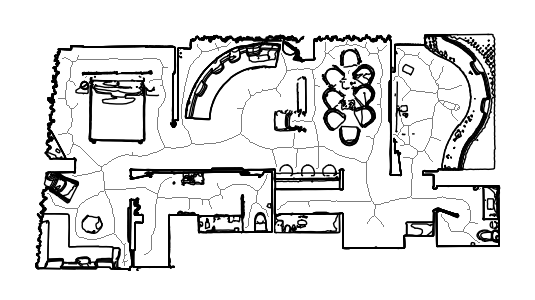
\includegraphics[width=\textwidth]{images/pose_estimator_skelethon_map.png}
		\caption{}
		\label{fig:pose_estimator_voronoi_graph}
	\end{subfigure}
	\hfil
	\begin{subfigure}[b]{0.49\linewidth}
		\centering
		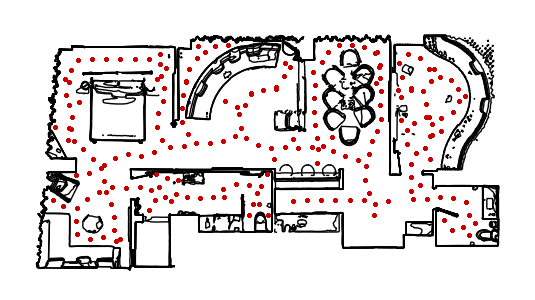
\includegraphics[width=\textwidth]{images/pose_estimator_subsampled.png}
		\caption{}
		\label{fig:pose_estimator_subsampled}
	\end{subfigure}
	\caption{The sub-sampling of the Voronoi graph.}
\end{figure}

\section{Dataset}

In our deep learning application, the dataset plays a crucial role to determine the final results. The virtualization environment used in this thesis (the modified version of Gibson described in Sec. \ref{sec:new_gibson_version}) offers three types of data during a simulation run: RGB images, depth data, and semantic information. The RGB images are tri-dimensional vectors $W \times H \times 3$, where $W = H$ and the last dimension contains the pixels' colors (red, green, and blue). Depth data are encoded in a bi-dimensional array with the same dimensions as the RGB images. In this way, a depth value is assigned to each pixel. Finally, semantic information is furnished in other RGB images, where the pixels are colored according to the object categories they belong to. Gibson provides 40 object categories (including doors), tagged with a numeric code. In the semantic images, the numerical code of each category is converted in an RGB color with the following procedure:

\begin{equation}
\label{eq:pareto mle2}
\begin{aligned}
B &= (\text{ID}) &\mod 256, \\
G &= (\text{ID} \gg 8) &\mod 256, \\
R &= (\text{ID} \gg 16) &\mod 256,
\end{aligned}
\end{equation}
where ID is the object category code and $\gg$ represents the bitwise right shift operation. 

In this section, we present the framework we develop to manage the vision dataset collected in this thesis. Then, we proceed by describing the dataset labeling procedure, reporting the difficulties encountered during this phase, and defining the final dataset's composition.

\subsection{The Dataset Management Framework}
\label{sec:generic_dataset}
In the initial phase of this thesis, we did not know what data characterized the collected examples. To overcome this uncertainty, we develop \textit{generic-dataset}\footnote{The generic-dataset repo: \url{https://github.com/micheleantonazzi/generic-dataset}.}, a configurable framework that automatically generates the code and the necessary classes to manage a dataset of any kind. This is possible using the \textit{meta-programming} paradigm offered by Python. Meta-programming is a technique in which computer programs have the ability to generate new code, create other programs, and modify their internal structure while running. This allows programs greater flexibility to efficiently handle new situations without recompilation. 

In Python, the meta-programming paradigm is implemented using \textit{decorators} and \textit{meta-classes}. A decorator allows programmers to modify the behavior of functions or classes. In other words, a decorator wraps an entity into a function in order to extend the behavior of the wrapped function or class, without permanently modifying it. The meta-classes, otherwise, represent a further implementation of meta-programming. In Python, everything is an object and classes are objects as well. A class in Python must have a type and it is an instance of another super-type, called meta-class. In simple terms, a meta-class is the definition of a class. The default meta-class which is responsible for making classes is called \textit{type}. Fig. \ref{fig:metaclass} visually explains the concept just reported: an object is an instance of a class and a class is an instance of a meta-class.

\begin{figure}[h!]
	\centering
	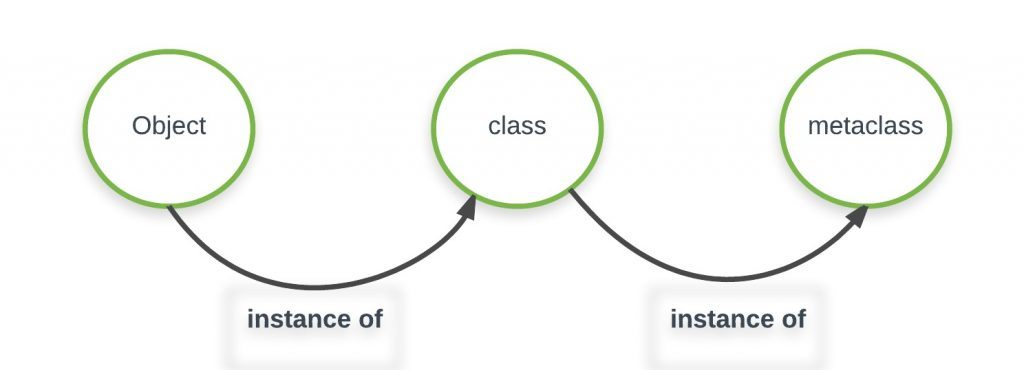
\includegraphics[width=\textwidth]{images/metaclass-hierarchy.jpeg}
	\caption{The hierarchy of objects, classes and meta-classes.}
	\label{fig:metaclass}
\end{figure}

Thanks to meta-programming, the programmer can write his own custom meta-classes to modify the way from which classes are generated by performing extra actions or injecting code. By exploiting this principle, the \textit{generic-dataset} framework offers an intuitive API that creates a custom class to model a particular examples' type of a generic dataset. To do this, this API, implemented by a \textsf{SampleGenerator} object, creates a meta-class according to the directions of the programmer, that defines the final desired class to deal with precise dataset's examples. In the constructor of \textsf{SampleGenerator}, the user specifies the name of the generated sample class and the label set. In this way, both regression or classification problems can be modeled. In a regression problem, the labels are real numbers and the label space is typically infinite. In this first case, the label set passed to the constructor must be empty. Otherwise, in a classification problem, the label set must contain all the possible labels that an example can assume. The programmer can also add data fields to the final generated class, specifying their name and type. In this case, the framework automatically generates useful methods to manipulate the custom fields (like getters and setters functions). Furthermore, the user can add custom methods to the final class in order to manipulate the example's fields. Finally, using the \textsf{generate\_sample\_class} method, \textsf{SampleGenerator}, the user obtains the generated custom class (which is an instance of the configured meta-class) which models a specific type of example. The instances of the generated class, that deal directly with the examples, are thread-safe. The generated class automatically implements this feature by assigning a lock to each data field. Then, each method is decorated with a function that acquires the locks of the fields used within each method before execution and then releases them. Also, the custom methods can be synchronized by specifying the name of the used fields.

Despite we did not know the exact final composition of our dataset, surely we will deal with image manipulation. To address this requirement,  \textit{generic-dataset} offers a useful utility to manipulate RGB images, that in Python are commonly stored in NumPy arrays. This utility, implemented by the \textsf{DataPipeline} class, generates an elaboration pipeline to modify a NumPy array. A pipeline consists of a series of operations performed consecutively that can be executed in CPU or in GPU according to the programmer's needs without changing the code. This is possible using CuPy\footnote{The CuPy web page: \url{https://cupy.dev/}.}, an open-source array library for GPU-accelerated computing with Python. The CuPy's interface is highly compatible with NumPy, allowing to write agnostic programs which can be executed in CPU or GPU by replacing the engine (NumPy or CuPy), without any code change. A pipeline can be customized by adding functions to modify the initial array and then executed using the \textsf{run} method. If the \textsf{use\_gpu} flag is set as \textsf{False}, the pipeline is synchronously executed in the CPU. Otherwise, if such flag is \textsf{True}, the operations are asynchronously performed by the GPU, so the user must synchronize the two elaboration units through the \textsf{get\_data} method. This mechanism is integrated into the class generated by \textsf{SampleGenerator}. It offers the possibility to automatically create an elaboration pipeline for the fields of the generated sample class. In addition, pipelines are protected with a dedicated lock which prevents data access and modification when during the execution of the correspondent pipeline.

The \textit{generic\_dataset} framework provides a mechanism to manage the dataset's persistence. It automatically organizes the folder hierarchy to store and organize the dataset and offers the necessary methods to save and load the examples. The classes generated by \textsf{SampleGenerator} are sub-type of \textsf{GenericSample} class, which provides a utility method to manage an example instance class of any kind. When the programmer adds a new field to the generated class, it must specify if it belongs to the dataset and, if so, it must provide the necessary functions for saving and loading such data type to the disk. The dataset folder hierarchy is organized as follows. The main directory is divided into sub-folders, that could specify different data categories or different moments in which the data are collected. Then, for a classification problem, the samples are divided into another level of sub-directories according to their label. Otherwise, in a regression task, the samples are saved in the same directory and the labels are stored in a dedicated file. Finally, the examples' fields are saved in different folders and the files inside them are named to reconstruct the acquisition order. More precisely, the file name contains two counters: the relative count and the absolute count. The first indicates the example's number based in its label's folder while the latter is the absolute count of the sample over all dataset. For a regression problem, these two values are equal because all examples belong to the same directory. Fig. \ref{fig:structuredataset} visually explain the folder hierarchy of a classification (Fig. \ref{fig:structureclassification}) and a regression (Fig. \ref{fig:structureregression}) problem. The entire dataset can be managed by an instance of \textsf{DatasetManager} class, while each folder at the first nesting level is controlled by an instance of \textsf{DatasetFolderManager}.

\begin{figure}[h!]
	\centering
	\begin{subfigure}[b]{0.5\textwidth}
		\dirtree{%
			.1 MAIN\_DATASET\_FOLDER.
			.2 FOLDER\_1.
			.3 0.
			.4 FIELD\_1.
			.5 field\_name\_rc\_ac.
			.5 field\_name\_rc\_ac.
			.5 \vdots.
			.4 FIELD\_2.
			.5 \vdots.
			.3 1.
			.4 FIELD\_1.
			.5 \vdots.
			.4 FIELD\_2.
			.5 \vdots.
			.2 FOLDER\_2.
			.3 \vdots.
			.2 \vdots.
		}
		\caption{}
		\label{fig:structureclassification}
	\end{subfigure}
	\begin{subfigure}[b]{0.4\textwidth}
		\dirtree{%
			.1 MAIN\_DATASET\_FOLDER.
			.2 FOLDER\_1.
			.3 LABEL.
			.4 label\_rc\_ac.
			.4 label\_rc\_ac.
			.4 \vdots.
			.3 FIELD\_1.
			.4 field\_name\_rc\_ac.
			.4 field\_name\_rc\_ac.
			.4 \vdots.
			.3 FIELD\_2.
			.4 field\_name\_rc\_ac.
			.4 field\_name\_rc\_ac.
			.4 \vdots.
			.2 FOLDER\_2.
			.3 \vdots.
			.2 \vdots.
		}
		\caption{}
		\label{fig:structureregression}
	\end{subfigure}
	\caption{The structure of a binary classification dataset (a) and a regression dataset (b). The files' names are are lowercase, where \textsf{rc} indicates the relative count of an example inside its label's folder, and \textsf{ac} represents the example's absolute count. }
	\label{fig:structuredataset}
\end{figure}


\subsection{Dataset Labeling and Composition}
\label{sec:dataset_labeling}
The labeling procedure in our robotic object detection task consists of dividing the positive examples (that contain the object of interest) from the negative ones and identifying the bounding boxes around the objects' instances. A vision dataset is mainly composed of RGB images, but it must specify the coordinates of the bounding boxes and their object categories in each image.

In our first dataset definition, each example is composed of all the data provided by Gibson: an RGB image, the semantic data, and the relative semantic information. The bounding boxes coordinates are not stored in dedicated files, but they are automatically calculated using  the semantic data provided by Gibson. To do this, we developed a dedicated function through the OpenCV's methods. At first, a semantic image is binarized assigning a precise color to the pixels that belong to a door and suppressing the others. Then, this function founds the contours in the binary image using the OpenCV's \textsf{findContours} method. Finally, a bounding box is created (through the \textsf{boundingRect} method of OpenCV) for each detected contour that contains a door. This function is useful because automatically designs the bounding boxes using semantic data.

Despite the usefulness of this method, we were forced to discard it after a few experiments. The main problems regard the semantic annotations. At first,  the knowledge provided by the semantic data was not enough informative to automatically label the dataset used in this thesis. This is because, semantic information does not specify the doors' status (open or closed) and does not include implicit doors, e.g. wall openings as described in Sec. \ref{sec:door_definition}. Furthermore, the Matterport3D scenes are categorized in an inaccurate and noisy way. The tagging procedure is extremely error-prone because the semantic information is provided by labeling the vertexes of the 3D environments' meshes. Specifically identifying objects in hundreds of thousands of vertices certainly leads to errors. Examining some collected examples, we assessed that some doors ended up on the wall (Fig. \ref{fig:wrong_box_1}) or were partially tagged. Furthermore, adjacent doors are difficult to distinguish and often are not clearly separated in the semantic image. Another problematic situation happens when the robot does not frame the upper door jamb. In this case, the two lateral sites are recognized as different doors because they do not share pixels in the semantic image (Fig. \ref{fig:wrong_box_2}). Due to these issues, automatically finding the bounding boxes through semantic annotation is unfeasible. As shown in Fig. \ref{fig:wrong_box}, the automatic labeling procedure using only the semantic data introduces noise that can degrade the doors detector's accuracy.

\begin{figure}[h!]
	\centering
	\begin{subfigure}[b]{\linewidth}
		\centering
		\begin{subfigure}[b]{0.32\linewidth}
			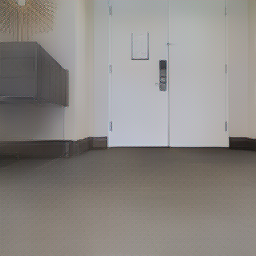
\includegraphics[width=\textwidth]{images/wrong_box_rgb_1.png}
		\end{subfigure}
		\hfil
		\begin{subfigure}[b]{0.32\linewidth}
			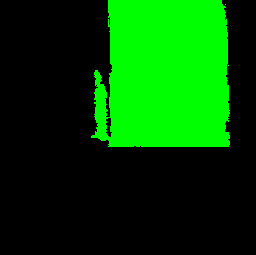
\includegraphics[width=\textwidth]{images/wrong_box_semantic_1.png}
		\end{subfigure}
		\hfil
		\begin{subfigure}[b]{0.32\linewidth}
			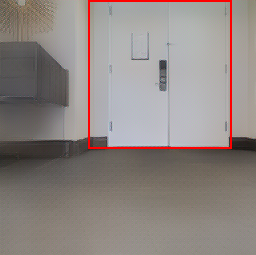
\includegraphics[width=\textwidth]{images/wrong_box_box_1.png}
		\end{subfigure}
		
		\caption{}
		\label{fig:wrong_box_1}
	\end{subfigure}
	\newline
	\begin{subfigure}[b]{\linewidth}
		\centering
		\begin{subfigure}[b]{0.32\linewidth}
			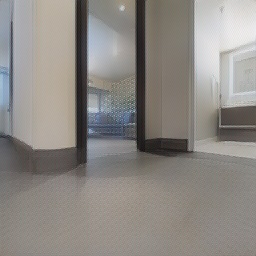
\includegraphics[width=\textwidth]{images/wrong_box_rgb_2.png}
		\end{subfigure}
		\hfil
		\begin{subfigure}[b]{0.32\linewidth}
			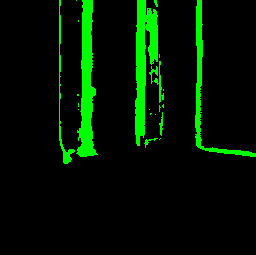
\includegraphics[width=\textwidth]{images/wrong_box_semantic_2.png}
		\end{subfigure}
		\hfil
		\begin{subfigure}[b]{0.32\linewidth}
			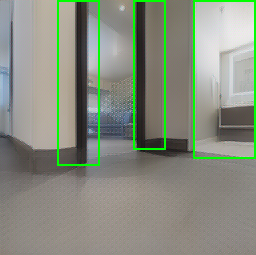
\includegraphics[width=\textwidth]{images/wrong_box_box_2.png}
		\end{subfigure}
		\caption{}
		\label{fig:wrong_box_2}
	\end{subfigure}

	\caption{Examples with inaccurate semantic annotations. Each row report two examples of wrong bounding boxes obtained through semantic data. From left to right, the figure shows the RGB image, the relative semantic data, and the bounding boxes derived from semantic information for each example.}
	\label{fig:wrong_box}
\end{figure}

The dataset acquisition has been performed using a hybrid method, which includes automatized procedures and the intervention of a human operator. At first, we acquired the dataset by saving all the data provided by Gibson (RGB and semantic images, and depth data). As mentioned in Sec. \ref{sec:solution}, a visual robotic dataset must contain also negative samples, so the first step concerns the discrimination between negative and positive data points. Despite the inaccuracy of the semantic data, we used them to separate the examples according to the door's presence: if the semantic image does not have pixel related to a door, the relative example is tagged as negative, as positive otherwise. Then, a human operator parses all the positive examples to define the bounding boxes and the related door's status (open or closed). For this purpose, we developed an intuitive visual tool inside the \textsf{scripts/data\_annotator.py} file of the \textit{gibson-env-utilities} package. This program loads each positive example and displays the bounding boxes extracted using the semantic data. The user can fix them by deleting the wrong bounding boxes and creating new ones, specifying also the doors' status. Some positive examples can not be used for training the doors detector module, e.g. if the robot is too close or too far to a door. In the first case, the RGB image depicts a uniform color not exposing the typical door's feature, likewise, in the second case, the doors appear as a small uniform rectangular. In particular, we discarded a door too close to the acquisition position considering the depth data: if the average distance is less that $0.30 m$, the bounding box is not displayed. Likewise, the doors too far with respect to the robot position are not considered if they cover less than $2,5\%$ of the total semantic image. In such situations, the tool we developed does not displays the bounding boxes. In this way, the user understands which doors should not be considered. In addition, the examples with no valid doors are discarded. The final doors dataset is composed of negative and positive examples. Each example is characterized by an RBG image, the depth data, and an array with contains the bounding boxes' coordinates and the related status. In the negative examples, the list of the bounding boxes is empty.

\begin{figure}[h!]
	\centering
	\begin{subfigure}[b]{\linewidth}
		\centering
		\begin{subfigure}[b]{0.4\linewidth}
			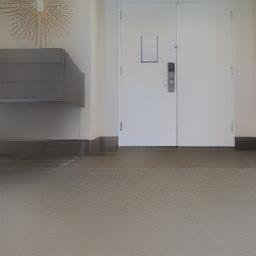
\includegraphics[width=\textwidth]{images/correct_box_rgb_1.png}
		\end{subfigure}
		\hfil
		\begin{subfigure}[b]{0.4\linewidth}
			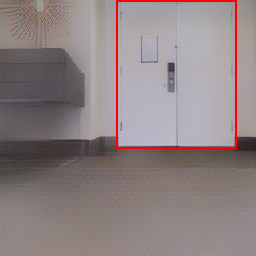
\includegraphics[width=\textwidth]{images/correct_box_box_1.png}
		\end{subfigure}
		\caption{}
		\label{fig:correct_box_1}
	\end{subfigure}
	\newline
	\begin{subfigure}[b]{\linewidth}
		\centering
		\begin{subfigure}[b]{0.4\linewidth}
			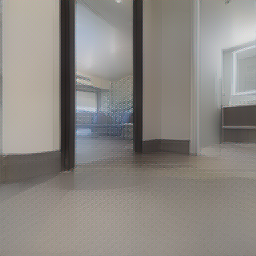
\includegraphics[width=\textwidth]{images/correct_box_rgb_2.png}
		\end{subfigure}
		\hfil
		\begin{subfigure}[b]{0.4\linewidth}
			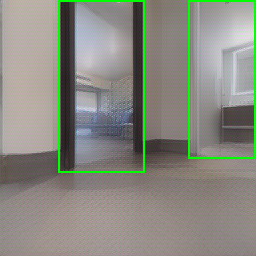
\includegraphics[width=\textwidth]{images/correct_box_box_2.png}
		\end{subfigure}
	\caption{}	
	\label{fig:correct_box_2}
	\end{subfigure}

	\caption{The fixed examples of Fig. \ref{fig:wrong_box}. These two data point belong to the final dataset labeled by a human operator.}
	\label{fig:correct_box}
\end{figure}

\section{Model Evaluator}
\label{sec:model_evaluator}
This module is responsible to evaluate the performance of the door's detector trained with the collected dataset. As mentioned in Sec. \ref{sec:goals}, we collect a dataset suitable for a robotic vision application, so it is composed of positive and negative examples (where the first contain open or closed doors while the latter do not contain any objects of interest). The metric we implement considers these two types of examples to better evaluate the model if used by an autonomous agent. 

The evaluation method proposed by this thesis is based on the metric of Pascal VOC challenge \cite{pascal}. This metric solves several issues related to the evaluation of models that perform object detection or segmentation. In an object detection task, images contain multiple object categories, and, in general,  multiple instances of the same object, so a standard approach to determine which one of the $m$ classes an image contains and where it can not be used. Furthermore, the prior distribution over different classes is significantly nonuniform so a
simple accuracy measure (percentage of correctly classified
examples) is not appropriate. During the evaluation, it is also necessary
to evaluate the trade-off between different types of classification error (e.g. false negative or false positive). The metric of the Pascal VOC challenge computes a separate ``score'' over each class to evaluate the model's performance in detecting each object category.  This metric calculates the interpolated Average Precision (AP), proposed by \citeauthor{averageprecision} in \cite{averageprecision}, for each class in the positive images, that are closed and open door in the context of this thesis. AP is determined by the area under the precision/recall curve in the $[0, 1]$ interval. Precision and recall are two measures that differently relate the true positive (TP), false positive (FP), and false negative (FN). In an object detection task where the predictions are bounding boxes, TPs are objects correctly recognized, FNs are objects not detected, while FPs are bounding boxes that do not correspond to any object. Precision measures how accurate the predictions are, i.e. the percentage of the correct predictions over the total number of objects to detect.

It requires as input the predicted bounding boxes with their confidence score.

\begin{equation}
\label{eq:precision}
Precision = \frac{TP}{TP + FP},
\end{equation}
where $TP + FP$ represents the total number of objects to detect. Otherwise, recall measures the goodness of detections performed by the model, relating the positive classifications with the total number of model's predictions.

\begin{equation}
\label{eq:recall}
Recall = \frac{TP}{TP + FN},
\end{equation}
where $TP + FN$ is the total number of predictions performed by the model. 
To discriminate true from false positive, detections (the predicted bounding boxes) are assigned to  ground-truth objects and judged to be true/false by measuring bounding box overlap. To be considered a correct detection, the area of overlap $a_0$ between the predicted bounding
box $B_p$ and  ground-truth bounding box $B_{gt}$ must exceed a threshold, set as 0.5 in the Pascal VOC challenge. This is the intersection over union (IoU) value:

\begin{equation}
\label{eq:iou}
a_0 = \frac{area(B_p \cap B_{gt})}{area(B_p \cup B_{gt})},
\end{equation}
where $B_p \cap B_{gt}$ denotes the intersection of the predicted and
 ground-truth bounding boxes and $B_p \cup B_{gt}$ their union. The area under the precision/recall curve is defined as the mean precision at a set of 11 equally spaced recall levels $ L = \{0, 0.1, 0.2, ..., 1\}$:

\begin{equation}
\label{eq:11-point}
	\text{AP} = \frac{1}{11} \sum_{r \in L} p_{interp}(r).
\end{equation}
The precision at each recall level $r$ is interpolated by taking
the maximum precision measured for a recall value that exceeds $r$:

\begin{equation}
p_{interp} (r) = \max_{\tilde{r} : \tilde{r} \geq r} p(\tilde{r}),
\end{equation}
where $p(\tilde{r})$ is the measured precision at recall $\tilde{r}$. 

The dataset of this thesis is composed of positive and negative images, that are treated differently by the evaluation method we propose. In the following paragraphs, we explain in detail how we evaluate the model's performance with the two different macro-categories of examples we collected (positive and negative). The evaluation procedure is implemented in a dedicated class, called \textsf{MyEvaluator}, contained in the main repository of this thesis. 

\paragraph*{Positive Images} The positive images are examples that contain doors to detect. As described in Sec. \ref{sec:door_definition}, we consider two possible statuses that a door can assume: \textsf{open} and \textsf{closed}. This means that the bounding boxes in the positive images belong to a set of two different object categories: $L = \{0, 1\}$. To discriminate the background bounding boxes, the doors detector we propose does not output a third label, but it assigns always a label in $L$ with  low accuracy, near to zero. 

The metric we use to evaluate the model's performance in the positive image is the same evaluation method used in Pascal VOC challenge \cite{pascal}. First of all, each image in the test set is classified by the model, and an instance of \textsf{MyEvaluator} stores the  ground-truth and the predicted bounding boxes. Then, the predicted bounding boxes are divided according to the object category the model assigns to them, in order to calculate an AP (average precision) score for each label (\textsf{open} and \textsf{closed} doors). The AP value is calculated as follow:

\begin{enumerate}
	\item the ground-truth and the predicted bounding boxes are filtered according to their confidence value: if a detection has confidence less than a threshold, called \textsf{confidence\_threshold}, it is discarded;
	\item the remaining bounding boxes are then descending ordered according to their confidence value;
	\item  following the order determined in the previous step, the module tries to match each predicted bounding box with a  ground-truth box. The matching procedure follows the next operations:
	\begin{itemize}
		\item each predicted bounding box is compared with the  ground-truth boxes of the same image, in order to find the one with the greater intersection under union (IoU) area (Eq. \ref{eq:iou});
		\item if the greater IoU area is overcome a threshold, called \textsf{iou\_threshold}, the predicted bounding box is matched with the corresponding  ground-truth box (if it has not been previously matched);
		\item the matching procedure determines the true positive (TP) and the false positive (FP) detections: each predicted bounding box matched with a  ground-truth box is considered a TP, while a detected bounding box with no match represents a FP;
	\end{itemize}
	\item when the matching procedure ends, the  ground-truth boxes not matched  are considered as false negative (FN);
	\item the true and false positives found during the matching operations are saved in order to compute the values of precision (Eq. \ref{eq:precision}) and recall (Eq. \ref{eq:recall}) at each matching step; 
	\item the final AP score is the area under the precision/recall curve Differently from the 11-points interpolation performed by the Pascal VOC metric, we interpolate such a curve with a variable set $L$ of points, considering local maximum of the precision/recall curve. This interpolation produces a more refined result than the 11-points interpolation performed in Pascal VOC metric expressed in Eq. \ref{eq:11-point}).
\end{enumerate} 

\begin{figure}[h!]
	\centering
	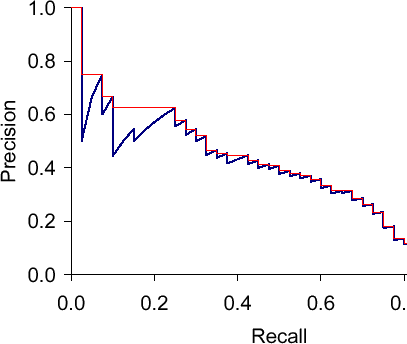
\includegraphics[width=0.8\textwidth]{images/interpolated.png}
	\caption{The interpolated precision/recall curve. The blue curve is the original curve while the red one is the interpolation. AP is the area under the interpolated curve.}
	\label{fig:interpolation}
\end{figure}

\paragraph{Negative Images} The negative images do not contain objects of interest, so they are evaluated in a different way. The procedure is inspired by the metric of Pascal VOC challenge \cite{pascal} with some refinements. As mentioned in Sec. \ref{sec:detr}, DETR outputs a fixed number of predictions for every image. The back bounding boxes do not have a dedicated label, but they are characterized by low accuracy. First of all, the predicted bounding boxes in the negative images lost the labels assigned by the model (\textsf{closed} or \textsf{open} doors). Then, the bounding boxes with a low confidence value are considered as TP (true positive) while those with a high confidence are FP (false positives). Finally, the metric we propose calculates the AP score on the average/precision curve. More in detail, the AP value in the negative images is computed as follow:

\begin{enumerate}
	\item the labels assigned by the model to the bounding boxes in the negative images are not considered. These bounding boxes take a unique label indicating all negative boxes (which we set to $ -1 $);
	\item the bounding boxes are grouped per image in which they are predicted;
	\item the negative images are ordered according to the sum over the single image of the predicted bounding boxes' confidence;
	\item following the order defined in the previous step, the evaluation method now processes each negative image to find the TP and the FP bounding boxes. If a bounding box has a confidence value less than \textsf{confidence\_threshold}, it is considered a true positive. Otherwise, a predicted bounding box in a negative image with a confidence score greater than \textsf{confidence\_threshold} is a false positive because it is considered a door. Both \textsf{iou\_threshold} and \textsf{confidence\_threshold} are hyper-parameters;
	\item the true and false positives are used to compute the values of precision (Eq. \ref{eq:precision}) and recall (Eq. \ref{eq:recall}) at each step; 
	\item the final AP score is the area under the precision/recall curve, calculated by interpolating such curve at every point (refining the 11-point interpolation performed in Pascal VOC metric expressed in Eq. \ref{eq:11-point}).
\end{enumerate}






